\documentclass[a4paper,11pt,oneside,titlepage,openright]{book}
\usepackage[english]{babel}
\usepackage[utf8]{inputenc}
\usepackage{indentfirst}
\usepackage[dvips]{graphicx}
\usepackage{amssymb}
\usepackage{amsmath}
\usepackage{latexsym}
\usepackage{amsthm}
\usepackage{amsfonts}
\usepackage{lettrine}
\usepackage{epsfig}
\usepackage{hyperref}
\usepackage{graphicx}
\usepackage{color}
\usepackage{xcolor}
\usepackage{courier}
\usepackage{caption}
\usepackage{mdwlist}
\usepackage{listings}
\usepackage[T1]{fontenc}
\usepackage{booktabs}
\usepackage{longtable}
\usepackage{pdflscape}
\usepackage{rotating}
%\usepackage[babel]{csquotes}
\usepackage{epigraph}
\usepackage{tabularx}
\usepackage[section]{placeins}
\usepackage[style=numeric-comp,useprefix,hyperref,backend=bibtex]{biblatex}

\bibliography{tex_files/bibliography/bibliography}
\pagestyle{headings}

\definecolor{editorGray}{rgb}{0.95, 0.95, 0.95}
\definecolor{editorOcher}{rgb}{1, 0.5, 0} % #FF7F00 -> rgb(239, 169, 0)
\definecolor{editorGreen}{rgb}{0, 0.5, 0} % #007C00 -> rgb(0, 124, 0)
\colorlet{punct}{red!60!black}
\definecolor{background}{HTML}{F5F5F5}
\definecolor{delim}{RGB}{20,105,176}
\colorlet{numb}{magenta!60!black}

\lstdefinelanguage{javascript}{
  morekeywords={typeof, new, true, false, catch, function, return, null, catch, switch, var, if, in, while, do, else, case, break},
  morecomment=[s]{/*}{*/},
  morecomment=[l]//,
  morestring=[b]",
  morestring=[b]'
}

\lstset{%
    % Basic design
    backgroundcolor=\color{background},
    basicstyle={\scriptsize\ttfamily},   
    frame=none,
    % Line numbers
    numbers=none,
    % xleftmargin={0.75cm},
    % numbers=left,
    % stepnumber=1,
    % firstnumber=1,
    % numberfirstline=true,
    % Code design   
    keywordstyle=\color{black}\bfseries,
    commentstyle=\color{darkgray}\ttfamily,
    ndkeywordstyle=\color{gray}\bfseries,
    stringstyle=\color{black},
    % Code
    language=html,
    alsolanguage=javascript,
    alsodigit={.:;},
    tabsize=2,
    showtabs=false,
    showspaces=false,
    showstringspaces=false,
    extendedchars=true,
    breaklines=true,        
    % Support for German umlauts
    literate=%
    {Ö}{{\"O}}1
    {Ä}{{\"A}}1
    {Ü}{{\"U}}1
    {ß}{{\ss}}1
    {ü}{{\"u}}1
    {ä}{{\"a}}1
    {ö}{{\"o}}1
}

\lstdefinelanguage{json}{
    basicstyle=\scriptsize\ttfamily,
    % Line numbers
    numbers=none,
    frame=none,
    % numbers=left,
    % numberstyle=\scriptsize,
    % stepnumber=1,
    % numbersep=8pt,
    % showstringspaces=false,
    % breaklines=true,
    % frame=lines,
    backgroundcolor=\color{background},
    literate=
     *{0}{{{\color{numb}0}}}{1}
      {1}{{{\color{numb}1}}}{1}
      {2}{{{\color{numb}2}}}{1}
      {3}{{{\color{numb}3}}}{1}
      {4}{{{\color{numb}4}}}{1}
      {5}{{{\color{numb}5}}}{1}
      {6}{{{\color{numb}6}}}{1}
      {7}{{{\color{numb}7}}}{1}
      {8}{{{\color{numb}8}}}{1}
      {9}{{{\color{numb}9}}}{1}
      {:}{{{\color{punct}{:}}}}{1}
      {,}{{{\color{punct}{,}}}}{1}
      {\{}{{{\color{delim}{\{}}}}{1}
      {\}}{{{\color{delim}{\}}}}}{1}
      {[}{{{\color{delim}{[}}}}{1}
      {]}{{{\color{delim}{]}}}}{1},
}

\DeclareCaptionFont{white}{\color{white}}
\DeclareCaptionFormat{listing}{\colorbox[cmyk]{0.43, 0.35, 0.35,0.01}{\parbox{\textwidth}{\hspace{15pt}#1#2#3}}}
\captionsetup[lstlisting]{format=listing,labelfont=white,textfont=white, singlelinecheck=false, margin=0pt, font={bf,footnotesize}}

\definecolor{lightgray}{rgb}{.9,.9,.9}
\definecolor{darkgray}{rgb}{.4,.4,.4}
\definecolor{purple}{rgb}{0.65, 0.12, 0.82}
\definecolor{Brown}{cmyk}{0,0.81,1,0.60}
\definecolor{OliveGreen}{cmyk}{0.64,0,0.95,0.40}
\definecolor{CadetBlue}{cmyk}{0.62,0.57,0.23,0}
\definecolor{lightlightgray}{gray}{0.9}

\linespread{1.5}

\newcommand{\minisizeurl}[1]{\footnotesize #1 \normalsize}

\newcommand{\terminale}{
    \lstset{language={}}
}

\newcommand{\javascript}{
    \lstset{
    language=JavaScript,
    backgroundcolor=\color{lightgray},
    extendedchars=true,
    basicstyle=\footnotesize\ttfamily,
    showstringspaces=false,
    showspaces=false,
    tabsize=2,
    breaklines=true,
    showtabs=false,
    captionpos=b
   }
}

\newcommand{\html}{
    \lstset{
        language=HTML,
        basicstyle=\ttfamily\footnotesize,
        keywordstyle=\color{OliveGreen},
        commentstyle=\color{gray},
        stepnumber=1,
        numbersep=5pt,
        backgroundcolor=\color{lightgray},
        frame=none,
        tabsize=2,
        captionpos=b,
        breaklines=true,
        breakatwhitespace=false,
        showspaces=false,
        showtabs=false,
        stringstyle=\color{red}\ttfamily,
        xleftmargin=17pt,
        framexleftmargin=17pt,
        framexrightmargin=5pt,
        framexbottommargin=4pt,
    }
}

\newcommand{\xml}{
    \lstset{
        language=XML,
        basicstyle=\ttfamily\footnotesize,
        keywordstyle=\color{OliveGreen},
        commentstyle=\color{gray},
        stepnumber=1,
        numbersep=5pt,
        backgroundcolor=\color{lightgray},
        frame=none,
        tabsize=2,
        captionpos=b,
        breaklines=true,
        breakatwhitespace=false,
        showspaces=false,
        showtabs=false,
        stringstyle=\color{red}\ttfamily,
        xleftmargin=17pt,
        framexleftmargin=17pt,
        framexrightmargin=5pt,
        framexbottommargin=4pt,
    }
}

\newcommand{\ext}{png}

% \newcommand{\def}[1]{{\em {\bfseries #1}}}

\hyphenation{sil-la-ba-zio-ne}
\hyphenation{del-le} \hyphenation{pa-ro-le}

% examples
\theoremstyle{plain}
\newtheorem{thm}{Teorema}[section]
\theoremstyle{definition}
\newtheorem{defn}{Definizione}[chapter]
\newtheorem{ex}{Esempio}[chapter]
\theoremstyle{remark}
\newtheorem{codifica}{Codifica}

\begin{document}

\baselineskip=12mm
\thispagestyle{empty}

\begin{figure}
\begin{center}
~~\centerline {
\psfig{file=images/logo/logo.png,width=5cm}}
\end{center}
\end{figure}

\vskip 1.40cm

\begin{center}
\large
Università degli Studi \textit{``Roma Tre''}\\
Facoltà di Ingegneria\\
Corso di Laurea Magistrale in Ingegneria Informatica\\
\end{center}

\vskip 1cm \Large

\begin{center}
Tesi di laurea magistrale
\end{center}

\vskip 1cm \baselineskip=10mm

\begin{center}
\textbf{{\em Techniques and tools based on HTML5 Web Components for storage and video streaming to support an e-learning platform}}\\
\end{center}

\vskip .4cm

\begin{center}
Laureando\\
{Alessandro Rastelli}\\
\end{center}

\vskip 1cm

\begin{center}
\large{
\begin{tabularx}{\textwidth}{>{\centering\arraybackslash}X >{\centering\arraybackslash}X}
  Relatore\\
  Prof.~Alberto Paoluzzi
\end{tabularx}
}
\large{
\begin{tabularx}{\textwidth}{>{\centering\arraybackslash}X >{\centering\arraybackslash}X}
  Correlatori\\
  Dott.~Enrico Marino, Dott.~Federico Spini\\
\end{tabularx}
}
\end{center}

\vskip 1.5cm

\centerline{Anno Accademico 2014/2015}

\normalsize


% \baselineskip=12mm
\thispagestyle{empty}

\begin{figure}
\begin{center}
~~\centerline {
\psfig{file=images/logo/logo.png,width=5cm}}
\end{center}
\end{figure}

\vskip 1.40cm

\begin{center}
\large
Università degli Studi \textit{``Roma Tre''}\\
Facoltà di Ingegneria\\
Corso di Laurea Magistrale in Ingegneria Informatica\\
\end{center}

\vskip 1cm \Large

\begin{center}
Tesi di laurea magistrale
\end{center}

\vskip 1cm \baselineskip=10mm

\begin{center}
\textbf{{\em Titolo della tesi}}\\
\end{center}

\vskip .5cm

\begin{center}
Laureando\\
{Nome Cognome}\\
\end{center}

\vskip 1cm

\begin{center}
\large{
\begin{tabularx}{\textwidth}{>{\centering\arraybackslash}X >{\centering\arraybackslash}X}
  Correlatori\\
  Dott.~Enrico Marino, Dott.~Federico Spini\\
\end{tabularx}
}
\end{center}

\vskip 1.5cm

\centerline{Anno Accademico 2014/2015}

\normalsize


% \baselineskip=12mm
\thispagestyle{empty}

\begin{figure}
\begin{center}
~~\centerline {
\psfig{file=images/logo/logo.png,width=5cm}}
\end{center}
\end{figure}

\vskip 1.40cm

\begin{center}
\large
Università degli Studi \textit{``Roma Tre''}\\
Facoltà di Ingegneria\\
Corso di Laurea Magistrale in Ingegneria Informatica\\
\end{center}

\vskip 1cm \Large

\begin{center}
Tesi di laurea magistrale
\end{center}

\vskip 1cm \baselineskip=10mm

\begin{center}
\textbf{{\em Titolo della tesi}}\\
\end{center}

\vskip .5cm

\begin{center}
Laureando\\
{Nome Cognome}\\
\end{center}

\vskip 1cm

\begin{center}
\large{
\begin{tabularx}{\textwidth}{>{\centering\arraybackslash}X >{\centering\arraybackslash}X}
  Correlatori\\
  Dott.~Enrico Marino, Dott.~Federico Spini\\
\end{tabularx}
}
\end{center}

\vskip 1.5cm

\centerline{Anno Accademico 2014/2015}

\normalsize


\newpage

\newpage\null\thispagestyle{empty}\newpage
\thispagestyle{empty}
\begin{flushright}
\null\vspace{\stretch{1}}
{\em Dedicated to my family} \\
{\em and ...}
\vspace{\stretch{2}}\null
\end{flushright}

% \newpage\null\thispagestyle{empty}\newpage
\thispagestyle{empty}
\begin{flushright}
\null\vspace{\stretch{1}}
{\em To my family} \\
{\em and ...}
\vspace{\stretch{2}}\null
\end{flushright}

% \newpage\null\thispagestyle{empty}\newpage
\thispagestyle{empty}
\begin{flushright}
\null\vspace{\stretch{1}}
{\em Dedicated to my family} \\
{\em and ...}
\vspace{\stretch{2}}\null
\end{flushright}

\frontmatter

\tableofcontents

\listoffigures

\chapter{Acknowledgements}
\label{cha:acknowledgements}

Firstly, I would like to express my sincere gratitude to our advisors, Enrico Marino and Federico Spini, for the continuous support of my project, for their patience, motivation, and immense knowledge. Besides my advisors, I would like to thank Prof. Alberto Paoluzzi for his supervision and the opportunity that he offered to me.

\chapter{Introduction}
\label{cha:introduction}

Once upon a time...

Section 1

Section 2

In conclusions...



% \chapter{Introduction}
\label{cha:introduction}

Once upon a time...

Section 1

Section 2

In conclusions...



% \chapter{Introduction}
\label{cha:introduction}

The arrival and diffusion of Internet has revolutionized the world in which we live in and has introduced, along with many other things, a new way of learning. With time, the first E-Learning services were devoloped and throughout the years they have evolved and are now commonly called MOOC (Massive Open Online Course).

The main difference between MOOC platforms today and in the past is that they generally offer open courses to anyone, in which the participation is free and they allow interactivity among the students.

The enormous potential of these systems has been noticed straight away and already in 2012 these services were about 100 and almost 700 in 2013, with an average of 2 new MOOCs per day.

It has been estimated that the turnover linked with E-Learning in 2012 alone was 35.6 billion dollars.\cite{gallico2015learning}.
Considering, however, the high number of platforms present, the market is very fragmented. Nonetheless, the most important part is taken up by the main platforms such as Coursera, EdX, Udacity, Udemy and SkillShare.

Some of the most prestigious universities, such as Standford, Harvard, Berkeley and MIT, use these platforms to deliver part of their own formative educational plans and extend their catchment area.
The courses offered cover various themes and are delivered directly to the professors of said universities.

The business model of these services consents the free access following the classic MOOC philosophy. A monetary fee is asked only if someone would like to have a certificate, which is released only after having passed an exam that verifies the actual learning level of the person.

MOOC has eliminated temporal and spatial barriers and has the merit of simplifying the access to a university training. They are often invoked as contributors when not directly makers of an actual revolution of the educational world.

During the last years, there has been a diffusion of an alternative model referred to the one introduced up until now: instead of an authoritative entity in the formation field, such as a prestigious university which delivers a course by one of their professors, some platforms are introducing the possibility of structuring an online course for anyone who is interested.

This is, for example, the case of Udemy, which has encountered a great success and has been used by many people who have published numerous courses on the platform. Some of these courses are accessible only after a payment has been made, thus becoming an actual profit for the professor.

\begin{figure}[htb] %  figure placement: here, top, bottom
 \centering
 
\includegraphics[width=0.7\linewidth]{images/introduction/mooc.png}\hfill
 \caption[Mooc image]{Mooc image}
 \label{fig:fourV}
\end{figure}


Despite the arrival of HTML5, video management is still very insidious. In fact, there isn't a video streaming standard that can ensure the fruition of the contents of the different web browsers and mobile devices.



In fact the lack of protocols shared by the vendor, together with the huge amount of data that must be managed by confronting video content, are a technological obstacle to face and overcome.

The creation of an e-learning service also requires a heavy investment to cover the costs of implementation, storage, and most importantly network traffic required for video content streaming.


The goal of this thesis work at the CVDLAB was to deepen methods and technologies to help overcome the technological obstacle identified in order to offer the opportunity to users and mainly companies to create their own E -learning platform.


For example, one use of the platform can be a big company that wants to create its own Academy section in which they can train the personnel without having to rely on third parties.

Finally, the concept of usability of the components based on the standard HTML5 Web Components was adopted, which greatly facilitated the creation of a final use case: X-Learning.


E-learning is a platform structured into two distinct parts: one part of administration that is addressed to a user who can manage the teacher staff and introduce courses, and another part for users who require the fruition content instead.


The thesis is divided into two parts, each of which consists of three chapters:
The first chapter provides an overview of the main existing MOOC platforms.

The second chapter describes the services used for the realization of the platform and a brief cost analysis.

The third chapter describes the technologies used for the development of the thesis project.

With the start of the second part of the thesis, the project gets more detailed, especially in the fourth chapter there will be an overview of the architecture and organization of the platform.

In the fifth chapter the focus is on core components made in the project and on how they were made.

The sixth and final chapter presents the conclusions and provides possible future developments, focusing on the issues put into production, not directly addressed during the thesis work.


\mainmatter

\part{Part 1}
\label{part:part_1}


\chapter{Massive open online course}
\label{cha:chapter_1}

This chapter describes MOOC’s world. In the first section a MOOCs overview is provided: what MOOCs are, what they are for and how they work. In the second section a classification of currently avalaible MOOCs is reported.

\section{MOOC overview}
\label{sec:mooc_overview}

This section consists of an overview about a massive open online course (MOOC). A MOOC is an online course aimed at unlimited participation and open access via the web. In addition to traditional course materials such as filmed lectures, readings, and problem sets, many MOOCs provide interactive user forums to support community interactions between students, professors, and teaching assistants (TAs). MOOCs are a recent and widely researched development in distance education which were first introduced in 2008 and emerged as a popular mode of learning in 2012.[Pappano, Laura. "The Year of the MOOC". The New York Times. Retrieved 18 April 2014.][Lewin, Tamar (20 February 2013). "Universities Abroad Join Partnerships on the Web". New York Times. Retrieved 6 March 2013.]. Early MOOCs often emphasized open-access features, such as open licensing of content, structure and learning goals, to promote the reuse and remixing of resources. Some later MOOCs use closed licenses for their course materials while maintaining free access for students.  [Wiley, David. "The MOOC Misnomer". July 2012] [Cheverie, Joan. "MOOCs an Intellectual Property: Ownership and Use Rights". Retrieved 18 April 2013.] [David F Carr (20 August 2013). "Udacity hedges on open licensing for MOOCs". Information Week. Retrieved 21 August 2013.][P. Adamopoulos, "What Makes a Great MOOC? An Interdisciplinary Analysis of Student Retention in Online Courses", ICIS 2013 Proceedings (2013) pp. 1–21 in AIS Electronic Library (AISeL)].

The first MOOCs emerged from the open educational resources (OER) movement. The term MOOC was coined in 2008 by Dave Cormier of the University of Prince Edward Island in response to a course called Connectivism and Connective Knowledge (also known as CCK08). CCK08, which was led by George Siemens of Athabasca University and Stephen Downes of the National Research Council, consisted of 25 tuition-paying students in Extended Education at the University of Manitoba.
Alongside the development of these open courses, other E-learning platforms emerged - such as Khan Academy, Peer-to-Peer University (P2PU), Udemy and ALISON - which are viewed as similar to MOOCs and work outside the university system or emphasize individual self-paced lessons.[Yuan, Li, and Stephen Powell. MOOCs and Open Education: Implications for Higher Education White Paper. University of Bolton: CETIS, 2013. pp. 7–8.][ "What You Need to Know About MOOCs". Chronicle of Higher Education. Retrieved 14 March 2013.][ "Open Education for a global economy".][ Booker, Ellis (30 January 2013). "Early MOOC Takes A Different Path". Information Week. Retrieved 25 July 2013.][Bornstein, David (11 July 2012). "Open Education For A Global Economy". New York Times. Retrieved 25 July 2013.].
According to The New York Times, 2012 became "the year of the MOOC" as several well-financed providers, associated with top universities, emerged, including Coursera, Udacity
In January 2013, Udacity launched its first MOOCs-for-credit, in collaboration with San Jose State University. In May 2013 the company announced the first entirely MOOC-based master's degree, a collaboration between Udacity, AT\&T and the Georgia Institute of Technology, costing \$7,000, a fraction of its normal tuition.["Georgia Tech, Udacity Shock Higher Ed With \$7,000 Degree". Forbes. 2012-04-18. Retrieved 2013-05-30.]






\section{Section 2}
\label{sec:chapter_1_section_2}

In this section...

In conclusions...



\chapter{Enabling Services}
\label{sec:Enabling Services}


This chapter presents the enabling services of thesis project.The first section provides a video platforms overview, and a classification of these. The following sections  provide an overview of the services adopted in thesis project and offered by AWS and also a overview of WebRTC and above all about PeerJs. The last section instead provides a cost analisys.

\section{Video platforms}
\label{sec:Video platforms}

The initial phase of the thesis project has been dedicated to the research of the different platforms of streaming video in order to highlight the strengths, differences and costs required. As stated previously, the next section briefly describes the features, services and costs of major video platforms, even though the final choice was to focus on the development of an independent video platform through the use of services offered by Amazon AWS.
\newpage
\subsection{JW Player}
\label{sec:JW Player}

\begin{figure}[htb]
 \centering
 \includegraphics[width=1.0\linewidth]{images/chapter2/jwtPLayer.png}\hfill
 \caption[JW player cost]{JW player cost}
 \label{fig:fourV}
\end{figure}

 JW Player is an open source solution, which allows anyone with a website to replace simple embedded videos from youtube with a real player, which is:

\begin{itemize}
\item Customizable
\item Reliable
\item Scalable
\item Compatible with different CMS via plugin
\item Free or Paid
\item Complete set API
JW Player supports playback of any format like the Adobe Flash Player along with HTML5, and reads compressed formats such as (FLV, H.264, MP4, VP8, WebM, MP3, AAC, JPG, PNG and GIF). JW Player also  supports content such as video streaming and live webcasting (RTMP, HTTP) and all CDN and switcher adaptive bitrate. These allow the distribution and playback of high-quality content.
\end{itemize}


\subsection{Video Wowza}
\label{sec:Video Wowza}
\begin{figure}[!htb]
 \centering
 \includegraphics[width=1.0\linewidth]{images/chapter2/wowza.png}\hfill
 \caption[Wowza cost]{Wowza cost}
 \label{fig:fourV}
\end{figure}

 The server Video Wowza is based on the platform streaming web TV Wowza Streaming Engine and is supplied with a control panel complete with:
\begin{itemize}

\item server settings Wowza
\item Quick links for different readers of Streaming
\item Player HTML5 to be included in the pages of your site (it works on fixed and mobile platforms)
\item Traffic statistics historical server
\item Statistics in real time of connected users with geolocation. The service is configurable in different bit rate depending on the needs of video quality:
\item 256 kbs - For a low resolution quality but accessible from mobile devices
\item 512 kbs - For a HQ quality standards equivalent to a normal television flow
\item 720 kbs - For HD quality videos
\item 1048 kbs - For a quality FULL HD video
\end{itemize}

You can send the video stream using any encoder that supports Wowza streaming server.



\subsection{Ustream}
\label{sec:Ustream}

\begin{figure}[!htb]
 \centering
 \includegraphics[width=1.0\linewidth]{images/chapter2/ustream.png}\hfill
 \caption[Ustream cost]{Ustream cost}
 \label{fig:fourV}
\end{figure}

Ustream is a broadcast platform for live streaming of events of any kind: from news conferences to product launches, from classes via teleconference to international protests.

Users can create a broadcast channel through their computer and a standard Web browser or a smartphone, via app for iOS and Android systems.
Users also can record their events and then load them on the platform, so that they can be broadcasted at another time. With the use of special cameras, Ustream makes it possible to stream HD video.
During the livestream viewers can interact with each other through chat and answer surveys and questionnaires posed by the organizers of the stream.

  

\section{Amazon AWS}
\label{sec:Amazon AWS}

Amazon Web Services (AWS) is a cloud-computing platform offered by Amazon.com and can be seen as a collection of remote computing services.
In 2006 Amazon understood that its infrastructure and its web services, which currently are used only for itself, could be shared with other companies who need a reliable infrastructure for their own business.

The services of AWS (Amazon Web Services) are divided and distributed in places completely autonomous and independent from each other, located in different places of the world. These services operate from 11 geographical regions (Regions) and in each region there are a number of infrastructure called availability zones.
The choice of the geographical area of Amazon AWS is very important because it influences the latency and the response time. Normally you should choose the closest geographical area since the costs for the same service are different from Brazil, USA, Europe, etc.
AWS is located in 11 geographical ``regions'': US East (Northern Virginia), where the majority of AWS servers are based,\cite{aws_stats1} US West (northern California), US West (Oregon), Brazil (São Paulo), Europe (Ireland and Germany), Southeast Asia (Singapore), East Asia (Tokyo and Beijing) and Australia (Sydney).

Each Region has multiple ``Availability Zones'', which are distinct data centers providing AWS services. Availability Zones are isolated from each other to prevent outages from spreading between Zones. Several services operate across Availability Zones (e.g., S3, DynamoDB) while others can be configured to replicate across Zones to spread demand and avoid downtime from failures. Amazon web services hold 1.79\% market share. As of December 2014, Amazon Web Services operated an estimated 1.4 Million servers across 28 availability zones \cite{aws_stats2}.


In conclusions...



\part{Part 2}
\label{part:part_2}


\chapter{Enabling Services}
\label{sec:Enabling Services}


This chapter presents the enabling services of thesis project.The first section provides a video platforms overview, and a classification of these. The following sections  provide an overview of the services adopted in thesis project and offered by AWS and also a overview of WebRTC and above all about PeerJs. The last section instead provides a cost analisys.

\section{Video platforms}
\label{sec:Video platforms}

The initial phase of the thesis project has been dedicated to the research of the different platforms of streaming video in order to highlight the strengths, differences and cost required. As already alluded in the next section briefly describes the features, services and costs of major video platforms, even though the final choice was to focus the argument on the development of a video platform independent through the use of services offered by Amazon AWS.

\subsection{JW Player}
\label{sec:JW Player}
 JW Player is an open source solution, allowing anyone with a website to replace the simple embedded from youtube with a real player:

\begin{itemize}
\item Customizable
\item Reliable
\item Scalable
\item Compatible with different CMS via plugin
\item Free or Paid
\item Complete set API
JW Player supports playback of any format the Adobe Flash Player and HTML5 and reads compressed formats such as (FLV, H.264, MP4, VP8, WebM, MP3, AAC, JPG, PNG and GIF), besides supports content such as video streaming and live webcasting (RTMP, HTTP) and all CDN and switcher adaptive bitrate allows the distribution and playback of high-quality content.
\end{itemize}


\begin{figure}[htb]
 \centering
 \includegraphics[width=1.0\linewidth]{images/chapter3/jwtPLayer.png}\hfill
 \caption[JW player cost]{JW player cost}
 \label{fig:fourV}
\end{figure}

\newpage 

\subsection{Video Wowza}
\label{sec:Video Wowza}
 The server Video Wowza is based on the platform streaming web TV Wowza Streaming Engine and is supplied with a control panel complete with:
\begin{itemize}

\item server settings Wowza
\item Quick links for different readers of Streaming
\item Player HTML5 to be included in the pages of your site (it works on fixed and mobile platforms)
\item Traffic statistics historical server
\item Statistics in real time of connected users with geolocation. The service is configurable in different bit rate depending on the needs of video quality:
\item 256 kbs - For a low resolution quality but accessible from mobile devices
\item 512 kbs - For a HQ quality standards equivalent to a normal television flow
\item 720 kbs - For HD quality videos
\item 1048 kbs - For a quality FULL HD video
\end{itemize}

You can send the video stream using any encoder that supports Wowza streaming server.


\begin{figure}[!htb]
 \centering
 \includegraphics[width=1.0\linewidth]{images/chapter3/wowza.png}\hfill
 \caption[Wowza cost]{Wowza cost}
 \label{fig:fourV}
\end{figure}

\subsection{Ustream}
\label{sec:Ustream}
 Ustream is a broadcast platform for live streaming of events of any kind: from news conferences to product launches, from classes via teleconference to international protests.

Users can create through their computer and a standard Web browser or a smartphone, via app for iOS and Android systems, broadcast channel.
Users also can register their events and then load them on the platform, so that they can be broadcast at a later date. With the use of special cameras also Ustream makes it possible to stream HD video.
During the direct viewers can interact with each other through chat and answer surveys and questionnaires posed by the organizers of the stream.

  
 \begin{figure}[!htb]
 \centering
 \includegraphics[width=1.0\linewidth]{images/chapter3/ustream.png}\hfill
 \caption[Ustream cost]{Ustream cost}
 \label{fig:fourV}
\end{figure}

\section{NodeJS}
\label{sec:nodejs}
This section provides an overview of NodeJs.
Node.js is an open source, cross-platform runtime environment for server- side and networking applications. Node.js applications are written in JavaScript and can be run within the Node.js runtime on OS X, Microsoft Windows, Linux, FreeBSD, NonStop,IBM AIX, IBM System z and IBM i. Its work is hosted and supported by the Node.js Foundation,a Collaborative Project at Linux Foundation.
\newline
Node.js provides an event-driven architecture and a non-blocking I/O API that optimizes an application’s throughput and scalability. These tech- nologies are commonly used for real-time web applications.
\newline
Node.js uses the Google V8 JavaScript engine to execute code, and a large percentage of the basic modules are written in JavaScript. Node.js contains a built-in library to allow applications to act as a Web server without software such as Apache HTTP Server, Nginx or IIS.
\newline
Node.js allows the creation of web servers and networking tools, using JavaScript and a collection of “modules” that handle various core functional- ity. Modules handle file system I/O, networking (HTTP, TCP, UDP, DNS, or TLS/SSL), binary data (buffers), cryptography functions, data streams , and other core functions. Node’s modules have a simple and elegant API, reducing the complexity of writing server applications.
Frameworks can be used to accelerate the development of applications, and common frameworks are Express.js, Socket.IO and Connect. Node.js applications can run on Microsoft Windows, Unix, NonStop and Mac OS X servers. Node.js applications can alternatively be written with CoffeeScript (an alternative form of JavaScript), Dart or Microsoft TypeScript (strongly typed forms of JavaScript), or any language that can compile to JavaScript.
Node.js is primarily used to build network programs such as web servers, making it similar to PHP and Python. The biggest difference between PHP and Node.js is that PHP is a blocking language (commands execute only after the previous command has completed), while Node.js is a non-blocking language (commands execute in parallel, and use callbacks to signal completion).
\newline
Node.js brings event-driven programming to web servers, enabling development of fast web servers in JavaScript. Developers can create highly scalable servers without using threading, by using a simplified model of event- driven programming that uses callbacks to signal the completion of a task. Node.js was created because concurrency is difficult in many server-side programming languages, and often leads to poor performance. Node.js connects the ease of a scripting language (JavaScript) with the power of Unix network programming.


\section{Web Components}
\label{sec:web_components}
This section provides an overview of Web  Components.
Web Components are a set of standards currently being produced by Google engineers as a W3C specification that allows for the creation of reusable widgets or components in web documents and web  applications.  The intention behind them is to bring component-based software engineering to the World Wide Web. The components model allows for encapsulation and interoperability of individual HTML  elements.
\newline
Support for Web Components is present in some WebKit-based browsers like Google Chrome and Opera and is in Mozilla Firefox (requires a manual configuration change). Microsoft’s Internet Explorer has not implemented any Web Components specifications yet.[1] Backwards compatibility with older browsers is implemented using JavaScript-based polyfills.\cite{tch_webcomp}

\begin{figure}[htb]
 \centering
 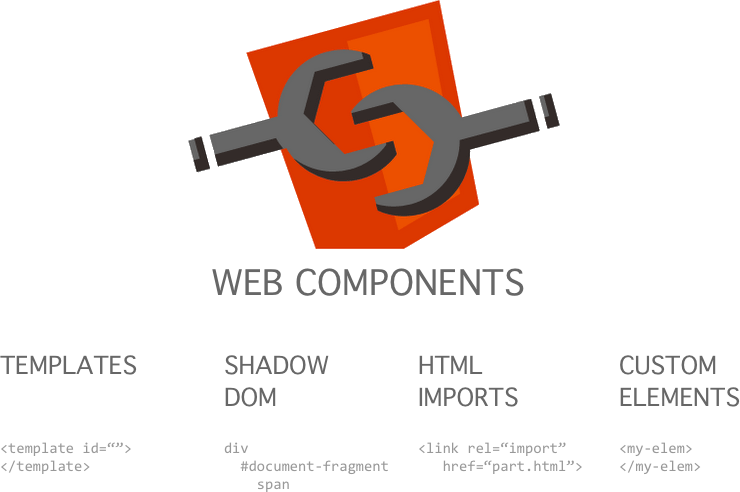
\includegraphics[width=1.0\linewidth]{images/chapter3/web_cmpts.png}\hfill
 \caption[Web Components]{Web Components}
 \label{fig:fourV}
\end{figure}
Web Components consist of 4 main elements which can be used separately or all together:
\begin{itemize}
\item Custom Elements: Custom Elements allow authors to define their own custom HTML elements. Authors associate JavaScript code with custom tag names, and then use those custom tag names as they would any standard tag.  Custom elements are still elements.  It is possible to create, use,
manipulate, and compose them just as easily as any standard <div> or <span> today.\cite{tch_custom}
\end{itemize}
\begin{itemize}
\item Shadow DOM: Shadow DOM addresses the lack of true DOM tree encapsulation when building components. With Shadow DOM, elements can get a new kind of node associated with them. This new kind of node is called a shadow root.  An element that has a “shadow root”  associated with it is called  a “shadow host”. The content of a shadow host isn’t rendered; the content of the shadow root is rendered instead.  Shadow DOM allows   a single node to express three subtrees:  light DOM, shadow DOM,  and composed DOM. Together, the light DOM and shadow DOM are referred to as the logical DOM. This is the DOM that the developer interacts with. The composed DOM is what the browser sees and uses to render the pixels on the  screen.\cite{tch_dom}
\newline
Structure of a Shadow DOM An element that has a shadow root asso- ciated with it is called shadow host. The shadow root can be treated as an ordinary DOM element, so it is possible to append arbitrary nodes to it. With Shadow DOM, all markup and CSS are scoped to the host element. In other words, CSS styles defined inside a Shadow Root won’t affect its parent document, CSS styles defined outside the Shadow Root won’t affect the main page.
\end{itemize}
\begin{itemize}
\item HTML Import: This webcomponents.js repository contains a  JavaScript  polyfill  for the HTML Imports specification. HTML Imports are a way to include and reuse HTML documents in other HTML documents. As <script> tags let authors include external JavaScript in their pages, imports let authors load full HTML resources. In particular, imports let authors include Custom Element definitions from external URLs.
\end{itemize}
\begin{itemize}
\item Templates: This specification describes a method for declaring inert DOM subtrees in HTML and manipulating them to instantiate document fragments with identical contents.
\end{itemize}

\section{X-Learning organization}
\label{sec:x-learning_organization}

  Durante la fase iniziale di analisi e progettazione si è evidenziata la necessità di suddividere il lavoro in due macro-blocchi public e admin. L’idea base è stata quella di delegare tutti compiti di creazione, gestione al lato admin e delegare invece la gestione della fruizione dei contenuti al lato client.
Inoltre questa scelta è dettata dalla volontà di rendere indipendenti tra di loro i vari componenti per permettere una maggiore flessibilità e garantire anche maggiore sicurezza posizionando per esempio il client in un server diverso da quello admin.
Il risultato finale ottenuto è quello di due piattaforme totalmente indipendenti che possono coesistere tra loro, permettendo massima autonomia e garantendo un elevato indice di coesione.


\begin{figure}[htbp] %  figure placement: here, top, bottom
 \centering
 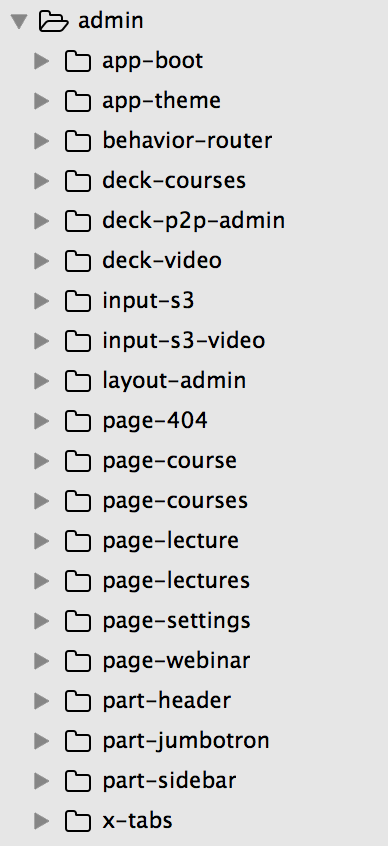
\includegraphics[width=0.5\linewidth]{images/chapter3/admin.png}\hfill
 \caption[admin hierarchy]{Admin hierarchy}
 \label{fig:fourV}
\end{figure}

\begin{figure}[htbp] %  figure placement: here, top, bottom
 \centering
 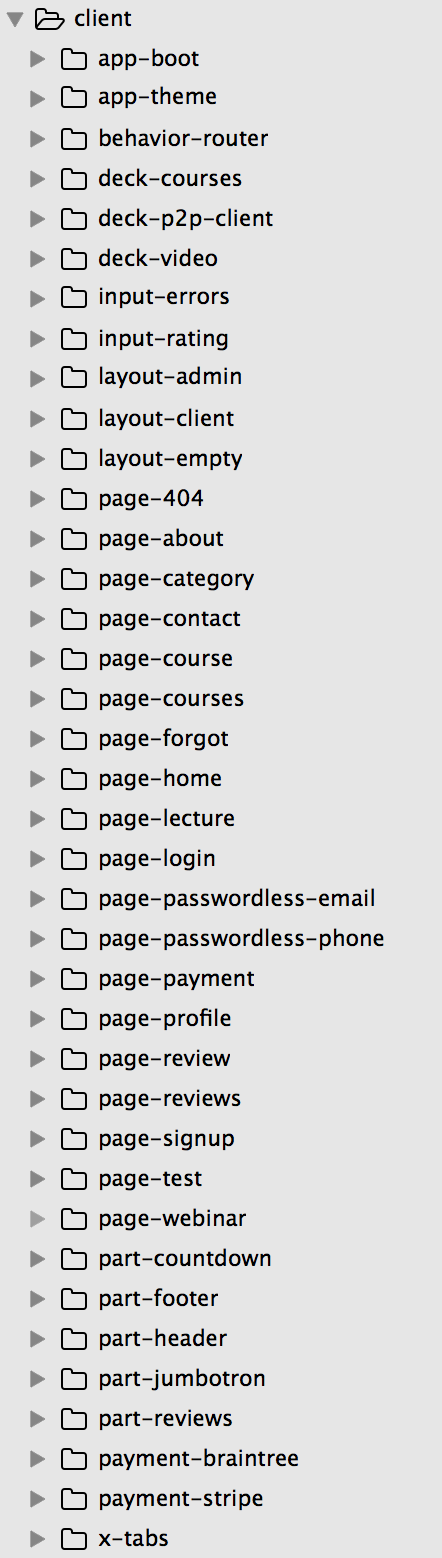
\includegraphics[width=0.5\linewidth]{images/chapter3/client.png}\hfill
 \caption[Client hierarchy]{Client hierarchy}
 \label{fig:fourV}
\end{figure}

\newpage

\section{NodeJS}
\label{sec:nodejs}
This section provides an overview of NodeJs.
Node.js is an open source, cross-platform runtime environment for server- side and networking applications. Node.js applications are written in JavaScript and can be run within the Node.js runtime on OS X, Microsoft Windows, Linux, FreeBSD, NonStop,IBM AIX, IBM System z and IBM i. Its work is hosted and supported by the Node.js Foundation,a Collaborative Project at Linux Foundation.
\newline
Node.js provides an event-driven architecture and a non-blocking I/O API that optimizes an application’s throughput and scalability. These tech- nologies are commonly used for real-time web applications.
\newline
Node.js uses the Google V8 JavaScript engine to execute code, and a large percentage of the basic modules are written in JavaScript. Node.js contains a built-in library to allow applications to act as a Web server without software such as Apache HTTP Server, Nginx or IIS.
\newline
Node.js allows the creation of web servers and networking tools, using JavaScript and a collection of “modules” that handle various core functional- ity. Modules handle file system I/O, networking (HTTP, TCP, UDP, DNS, or TLS/SSL), binary data (buffers), cryptography functions, data streams , and other core functions. Node’s modules have a simple and elegant API, reducing the complexity of writing server applications.
Frameworks can be used to accelerate the development of applications, and common frameworks are Express.js, Socket.IO and Connect. Node.js applications can run on Microsoft Windows, Unix, NonStop and Mac OS X servers. Node.js applications can alternatively be written with CoffeeScript (an alternative form of JavaScript), Dart or Microsoft TypeScript (strongly typed forms of JavaScript), or any language that can compile to JavaScript.
Node.js is primarily used to build network programs such as web servers, making it similar to PHP and Python. The biggest difference between PHP and Node.js is that PHP is a blocking language (commands execute only after the previous command has completed), while Node.js is a non-blocking language (commands execute in parallel, and use callbacks to signal completion).
\newline
Node.js brings event-driven programming to web servers, enabling development of fast web servers in JavaScript. Developers can create highly scalable servers without using threading, by using a simplified model of event- driven programming that uses callbacks to signal the completion of a task. Node.js was created because concurrency is difficult in many server-side programming languages, and often leads to poor performance. Node.js connects the ease of a scripting language (JavaScript) with the power of Unix network programming.


\section{Web Components}
\label{sec:web_components}
This section provides an overview of Web  Components.
Web Components are a set of standards currently being produced by Google engineers as a W3C specification that allows for the creation of reusable widgets or components in web documents and web  applications.  The intention behind them is to bring component-based software engineering to the World Wide Web. The components model allows for encapsulation and interoperability of individual HTML  elements.
\newline
Support for Web Components is present in some WebKit-based browsers like Google Chrome and Opera and is in Mozilla Firefox (requires a manual configuration change). Microsoft’s Internet Explorer has not implemented any Web Components specifications yet. Backwards compatibility with older browsers is implemented using JavaScript-based polyfills.\cite{tch_webcomp}

\begin{figure}[htb]
 \centering
 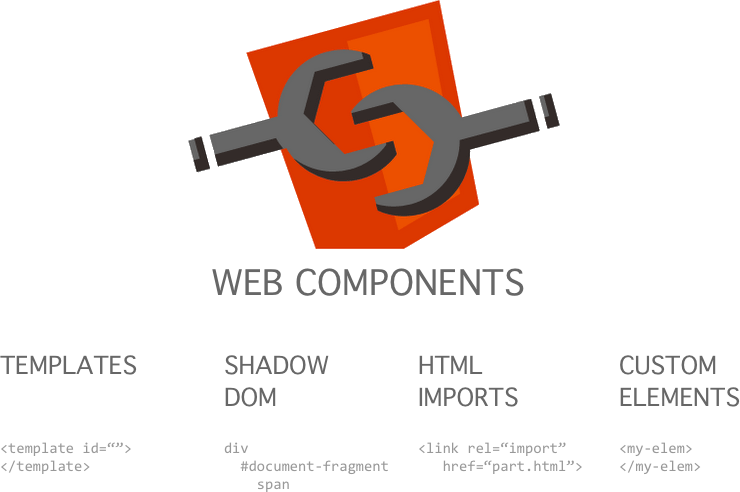
\includegraphics[width=1.0\linewidth]{images/chapter3/web_cmpts.png}\hfill
 \caption[Web Components]{Web Components}
 \label{fig:fourV}
\end{figure}
Web Components consist of 4 main elements which can be used separately or all together:
\begin{itemize}
\item Custom Elements: Custom Elements allow authors to define their own custom HTML elements. Authors associate JavaScript code with custom tag names, and then use those custom tag names as they would any standard tag.  Custom elements are still elements.  It is possible to create, use,
manipulate, and compose them just as easily as any standard <div> or <span> today.\cite{tch_custom}
\end{itemize}
\begin{itemize}
\item Shadow DOM: Shadow DOM addresses the lack of true DOM tree encapsulation when building components. With Shadow DOM, elements can get a new kind of node associated with them. This new kind of node is called a shadow root.  An element that has a “shadow root”  associated with it is called  a “shadow host”. The content of a shadow host isn’t rendered; the content of the shadow root is rendered instead.  Shadow DOM allows   a single node to express three subtrees:  light DOM, shadow DOM,  and composed DOM. Together, the light DOM and shadow DOM are referred to as the logical DOM. This is the DOM that the developer interacts with. The composed DOM is what the browser sees and uses to render the pixels on the  screen.\cite{tch_dom}
\newline
Structure of a Shadow DOM An element that has a shadow root asso- ciated with it is called shadow host. The shadow root can be treated as an ordinary DOM element, so it is possible to append arbitrary nodes to it. With Shadow DOM, all markup and CSS are scoped to the host element. In other words, CSS styles defined inside a Shadow Root won’t affect its parent document, CSS styles defined outside the Shadow Root won’t affect the main page.
\end{itemize}
\begin{itemize}
\item HTML Import: This webcomponents.js repository contains a  JavaScript  polyfill  for the HTML Imports specification. HTML Imports are a way to include and reuse HTML documents in other HTML documents. As <script> tags let authors include external JavaScript in their pages, imports let authors load full HTML resources. In particular, imports let authors include Custom Element definitions from external URLs.
\end{itemize}
\begin{itemize}
\item Templates: This specification describes a method for declaring inert DOM subtrees in HTML and manipulating them to instantiate document fragments with identical contents.
\end{itemize}

\section{Strongloop Loopback}
\label{sec:strongloop_loopback}
This section provides an overview of LoopBack.
\newline
Built on top of the open source LoopBack framework, the StrongLoop API Platform is the first end-to-end platform for the full API lifecycle that allows to visually develop REST APIs in Node and get them connected to new and legacy data. In addition, the API Platform features built-in mBaaS features like push and offline sync, plus graphical tools with DevOps features for clustering, profiling and monitoring Node apps.
\newline
LoopBack generates model API from the models schemas, to let CRUD operations on models.
LoopBack models automatically have a standard set of HTTP endpoints that provide REST APIs for create, read, update, and delete (CRUD) operations on model data:
\begin{itemize}
\item \textbf{POST /Model} — Create a new instance of the model and persist it into the data source.
\item \textbf{GET /Model} — Find all instances of the model matched by filter from the data source.
\item \textbf{PUT /Model} — Update an existing model instance or insert a new one into the data source.
\item \textbf{PUT /Model/id} — Update attributes for a model instance and persist it into the data source.
\item \textbf{GET /Model/id} — Find a model instance by id from the data source.
\item \textbf{DELETE /Model/id } — Delete a model instance by id from the data source.
\item \textbf{GET /Model/count} — Count instances of the model matched by where from the data source.
\item \textbf{GET /Model/findOne} — Find first instance of the model matched by filter from the data source.
\item \textbf{POST /Model/update} — Update instances of the model matched by where from that data source.
\end{itemize}
\begin{figure}[htb]
 \centering
 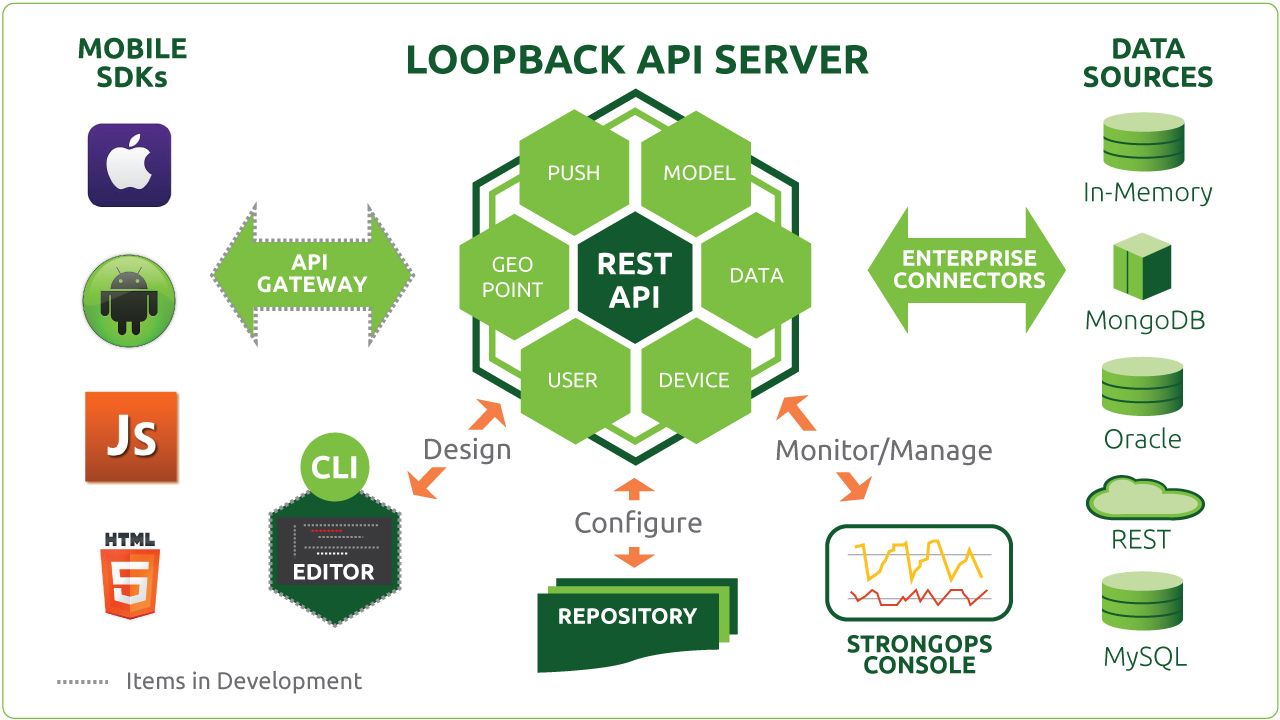
\includegraphics[width=0.9\linewidth]{images/chapter3/loopback_architecture.jpg}\hfill
 \caption[Loopback Architecture]{Loopback Architecture}
 \label{fig:loopback_architecture}
\end{figure}
A LoopBack model represents data in backend systems such as databases, and by default has both Node and REST APIs. Additionally, developer can add functionality such as validation rules and business logic to models. Every LoopBack application has a set of predefined built-in models such as User, Role, and Application. Developer can extend built-in models to suit application’s needs.
\newline
The model JSON file defines models, relations between models, and access to models.
\begin{lstlisting}[language=json]
{
  {
  "name": "ModelName", // See Top-level properties below "description": "A Customer model representing our customers.", "base": "User",
  "idInjection": false,
  "strict": true,
  "options": { ... }, // See Options below
  "properties": { ... }, // See Properties below
  "validations": [...], // See Validations below
  "relations": {...}, // See Relations below
  "acls": [...], // See ACLs below
  "scopes": {...}, // See Scopes below
   "http": {"path": "/foo/mypath"}
  }
}
\end{lstlisting}
Where:
\begin{itemize}
\item “name”: Name of the model.
\item “description”: Optional description of the model.
\item “base”: Name of another model that this model extends. The model will “inherit” properties and methods of the base model.
\item “IdInjection”: Whether to automatically add an id property to the model:
\begin{itemize}
\item true - id property is added to the model automatically. This is the default.
\item false - id property is not added to the model.
\end{itemize}
\item “strict”: Specifies whether the model accepts only predefined properties or not. One of:
\begin{itemize}
\item true - Only properties defined in the model are accepted. Used to ensure that the model accepts only predefined properties.
\item false - The model is an open model and accepts all properties, including ones not predefined in the model. This mode is useful to store free-form JSON data to a schema-less database such as MongoDB.
\item validate - The unknown properties will be reported as validation errors.
\item throw - Throws an exception if properties not defined for the model are used in an operation.
\item undefined - Defaults to false unless the data source is backed by a relational database such as Oracle or MySQL.
\item “options”: JSON object that specifies model options.
\item “properties”: JSON object that specifies the properties in the model.
\item “relations”: Object containing relation names and relation definitions.
\item “acls”: Set of ACL specifications that describes access control for the model.
\end{itemize}
\end{itemize}
The API can be extended: the developer can add remote functions to models or add hooks to existing API to add custom behavior before and/or after the API handler (to pre-process the re-quest and/or post-process the response). The resulting API is RESTful, cookie free, signed by authentica- tion token. By default, applications have a built-in model that represents a user, with properties username, email and password and role for authentica- tion and authorization. Loopback also introduces an indirection layer that allows to choose from almost all particular DBMS to be used.
In Chapter Two the technologies used for developing this work, have been described. Each technology has been described in realtion to its function and its use in the project.


\chapter{Video Management:S3 Component}
\label{cha:Video Management:S3 Component}

This chapter presents the core of the thesis project: X-Learning.
The first section provides a project’s overview, giving reasons of development, listing benefits and functions. The second section shows the X-Learning architectural stack and the reasons why these technologies have been chosen. The last section presents the development methodology that has been employed for the project.

\section{X-Learning overview}
\label{sec:x_learning_overview}

X-Learning is a platform to build full-stack Javascript NodeJS API-centric HTML5 based Single Page Application with Web Components via Polymer- Project. X-learning is composed of guidelines, methodology and a library of elements. The document driven web development methodology and guidelines allow to build a very structured and usable Single Page Application. 
“Everything is an element, even a service” is the philosophy of the project. The joint use of Web Components and Strongloop Loopback framework following the document driven web development methodology allowed to create vertical widget that influence every level of the stack. With a descriptive implementation it is possible to give life to API, on the server side, and visual and functional widget on the client side. A Web Application is essentially built by composing elements together. The Huge benefits coming from web components environment are reusability and access to reusable code.In X-Learning guidelines this pattern is applied to every kind of element.

.............

\section{X-Learning  Architecture}
\label{sec:x-learning_architecture}

A Web application developed by using the x-project toolkit, is a full stack JavaScript  Single  Page Application.


\subsection{Server side}
\label{subsec:server_side}

On the server side, an X-Learning app is based on NodeJS (see 2.4) used to create the server environment, MongoDB (see 2.5) used to storage data, and the Web framework Loopback by Strongloop (see 2.6).
Node.js is a JavaScript runtime built on Chrome’s  V8  JavaScript  engne. Node.js uses an event-driven, non-blocking I/O model that makes it lightweight and efficient. Node.js’ package ecosystem, npm, is the largest ecosystem of open source libraries in the world. NodeJS lets to create a vertical full-stack application in Javascript. The NodeJS asynchronous development scheme increases performances of web applications, by using downtime caused  by  HTTP requests.
LoopBack generates model API from the models schemas, to let CRUD operations on models. Loopback is the core of the X-Learning server-side. Document oriented API definition guarantees easiness and speed in API creation. Moreover, Loopback, is fully compatible with several DBMS thanks to connectors.
MongoDB is a cross-platform document-oriented database.  Classified as a NoSQL database, MongoDB eschews the traditional table-based relational database structure in favor of JSON-like documents with dynamic schemas. The document-oriented being of MongoDB allows to horizontal scale in really easy way. Moreover, document models, that replace relational database’s rows, are schemaless: this feature gives to MongoDB project high levels of flexibility and manageability.

\subsection{Client side}
\label{subsec:client_side}

On the client side, an X-Learning app is based on HTML5 Web Components via Polymer-Project by Google. It is a set of Polymer elements for local routing, API request, forms, lists, style and admin panels (as listed further    4.6).
Polymer-Project is one of the most important emerging realities of the moment. Google team has heavily focused his forces on code reusability and on separation between behavior, presentation and content.  Code reusability is a direct effect of Web Components structure: the creation of widget that can be completely indipendent facilitates code reuse.
Finally, the union between Polymer and Strongloop has been topped by the creation of the document oriented development process described below 4.5.

\begin{figure}[htb] %  figure placement: here, top, bottom
 \centering
 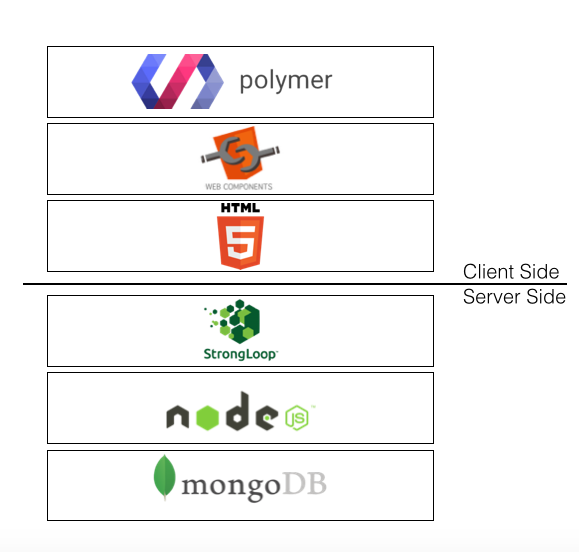
\includegraphics[width=1.0\linewidth]{images/chapter4/XPR_stack.png}\hfill
 \caption[X-learning Architectural Stack]{X-Learning Architectural Stack}
 \label{fig:fourV}
\end{figure}

\section{X-Learning design}
\label{sec:x-learning_design}

Durante la fase iniziale di analisi e progettazione si è evidenziata la necessità di suddividere il lavoro in due macro-blocchi public e admin. L’idea base è stata quella di delegare tutti compiti di creazione, gestione al lato admin e delegare invece la gestione della fruizione dei contenuti al lato client.
Inoltre questa scelta è dettata dalla volontà di rendere indipendenti tra di loro i vari componenti per permettere una maggiore flessibilità e garantire anche maggiore sicurezza posizionando per esempio il client in un server diverso da quello admin.


The process to build a web application based on x-learning toolkit consists of the following four steps: models schemas definition, HTTP RESTful API definition, UI components definition and UI components  assembly.


\subsection {Models schemas definition}
\label{subsec:models_schemas_definitio}


A description of entities, properties, relations and data access policies are defined as JSON  documents.
As to a learning platform, the essential entities to be modelled are the following: Course, Lecture, Video and Teacher(Member).


\subsubsection{ Model - Manager}

The model Manager represents the Aministrator of platform and course creator. Its features are: role, fullname, location and is\_main\_Admin can be true o false if he is the amministrator or invitable author. The Manager has relations teaching with courses.

\begin{lstlisting}[language=json]
{
  "name": "Manager",
  "plural": "managers",
  "base": "InvitableUser",
  "properties": {
    "role": { "type": "string", "enum": [ "admin", "editor", "author"]
    },
    "fullname": { "type": "string" },
    "location": { "type": "string" },
    "is_main_admin": { "type": "Boolean", "required": false }
  },
  "relations": {
    "teaching": { "type": "hasMany", "model": "Course", "foreignKey": "teacher_id" }
}
\end{lstlisting}


\subsubsection{ Model - Member}

The model Member represents students of other course. Its features are: name, lastname, email.gender,photo,phone number,location and date. The Member has relations learning with course.

\begin{lstlisting}[language=json]
{
  "name": "Member",
  "base": "User",
  "properties": {
    "first_name": { "type": "String" },
    "last_name": { "type": "String" },   
    "birthday": { "type": "Date" },
    "email": { "type": "String" },
    "gender": { "type": "String" },
    "password": { "type": "String" },
    "photo": { "type": "String" },
    "location": { "type": "String" },
    "phone": { "type": "Number" }
  },
  "relations": {
    "learning": { "type": "hasAndBelongsToMany", "model": "Course" },
    "teaching": { "type": "hasMany", "model": "Course" }
  }
}
\end{lstlisting}


\subsubsection{ Model - Course}

The model Course defines the main element structure that must be published. Main features are: title, cost, documentation, publish and publication date. This model has relations with teacher, students, category, lectures and webinars models.


\begin{lstlisting}[language=json]
{
  "name": "Course",
   "properties": { "title": { "type": "String" },
    "description": { "type": "String" },
    "date": { "type": "Date" },
    "cover": { "type": "String" },
    "language": { "type": "String" },
    "cost": { "type": "Number" },
    "publish": { "type": "Boolean" },
    "documents": { "type": "Array" },
    "skill": { "type": "Array" }
  },
  "relations": {
    "category": { "type": "belongsTo", "model": "Category" },
    "teacher": { "type": "belongsTo", "model": "Member" },
    "lectures": { "type": "hasMany", "model": "Lecture" },
    "webinars": { "type": "hasMany", "model": "Webinar" },
    "students": { "type": "hasAndBelongsToMany", "model": "Member" }

\end{lstlisting}

\subsubsection{ Model - Lecture}

The model Lecture defines the single lecture into a determinate course. Main features are: title, description. This model has relations with course, video.


\begin{lstlisting}[language=json]
{
  "name": "Lecture",
  "properties": {
    "title": { "type": "String" },
    "description": { "type": "String" }
  },
  "relations": {
    "course": { "type": "belongsTo","model": "Course" },
    "video": { "type": "hasOne", "model": "Video" }
  }

\end{lstlisting}

\subsubsection{ Model - Video}

The model Video defines the video object belong to lecture. Main features are: title, url and duration of its. This model has relations with lecture.


\begin{lstlisting}[language=json]
{
  "name": "Video",
  "properties": {
    "title": { "type": "String" }
    "url": { "type": "String" },
    "duration": { "type": "Number" }
  },
  "relations": {
    "lecture": { "type": "belongsTo", "model": "Lecture" }
  }
}

\end{lstlisting}


\subsection {HTTP RESTful API definition}
\label{subsec:HTTP_RESTful_API_definition}

CRUD operations on models are automatically generated by the web framework (on the basis of input JSON documents) and further custom actions can be defined. All of them are exposed as HTTP RESTful API.
These models result in the following HTTP RESTful API, automatically generated by Loopback server.

\subsubsection{ Members API}
\begin{itemize}
\item \textbf{GET /api/Members} Find all instances of the model matched by filter from  the  data source.
\item \textbf{POST /api/Members} Update an existing model instance or insert a new one into the data  source.
\item \textbf{PUT /api/Members} Create a new instance of the model and persist it into the data source.
\item \textbf{DELETE /api/Members/id} Delete a model instance by id from the data source.
\item \textbf{GET / Members/id/teaching} {\color{red}Queries teacher course of model.}

\item \textbf{GET / Members/id/learning} {\color{red} Queries follow course of model.}

\item \textbf{POST /api/changeEmail} Change email of a model instance.
\item \textbf{POST /api/changePassword} Change password of a model instance.
\item \textbf{GET /api/count Count} instances of the model matched by where from the  data source.
\item \textbf{POST /api/login} Login a user with username/email and password.
\item \textbf{POST /api/logout} Logout a user with access   token.
\item \textbf{POST /api/reset} Reset password for a user with email.
\item \textbf{POST /api/update} Update instances of the model matched by where from the data source.
\end{itemize}

\subsubsection{ Course API}
\begin{itemize}
\item \textbf{PUT /Courses} Update an existing model instance or insert a new one into the data  source.
\item \textbf{GET /Courses} Find all instances of the model matched by filter from the data  source.
\item \textbf{POST / Courses} create a new instance and persist it into the data source.
\item \textbf{GET / Courses/id/lectures} Queries lectures of course.
\item \textbf{POST / Courses/id/lectures} Creates a new instance in lectures of  this model.
\item \textbf{DELETE / Courses/id/lectures} Deletes all lectures of this model.

\item \textbf{GET / Courses/id/webinars} Queries webinars of course.
\item \textbf{POST / Courses/id/webinars} Creates a new instance in webinars of  this model.
\item \textbf{DELETE / Courses/id/webinars} Deletes all webinars of this model.

\item \textbf{GET / Courses/id/students} Queries students of course.
\item \textbf{POST / Courses/id/students} Creates a new instance in students of  this model.
\item \textbf{DELETE / Courses/id/students} Deletes all students of this model.
\end{itemize}


\subsubsection{ Lectures API}
\begin{itemize}
\item \textbf{GET /api/Lectures} Find all instances of the model matched by filter from  the  data source.
\item \textbf{POST /api/Lectures} Update an existing model instance or insert a new one into the data  source.
\item \textbf{PUT /api/Lectures} Create a new instance of the model and persist it into the data   source.
\item \textbf{DELETE /api/Lectures/id} Delete a model instance by id from the data source.
\item \textbf{GET /api/Lectures/id/course} Fetches belongsTO relation course.

\item \textbf{GET /api/Lectures/id/video} Fetches belongsTO relation video.
\item \textbf{GET /api/Lectures/count} Count instances of the model matched by where from the data  source.
\end{itemize}

\subsubsection{ Images API}

\begin{itemize}
\item \textbf{POST /Model}
\item \textbf{POST /Images} create a new instance and persist it into the data source.
\item \textbf{PUT /Images} Update an existing model instance or insert a new one into the data source.
\item \textbf{GET /Images} Find all instances of the model matched by filter from the  data source.
\item \textbf{POST /Images/upload} Upload a new instance into data source.
\item \textbf{GET /Images/id} Find a model instance by id from the data source
\item \textbf{PUT /Images/id} Update attributes of a model instance and persist it into the data source.
\item \textbf{DELETE /Images/id} Deletes a model instance by id from the data 
source.
\end{itemize}

\subsubsection{ Videos API}
\begin{itemize}
\item \textbf{POST /Videos} create a new instance and persist it into the data source.
\item \textbf{PUT /Videos} Update an existing model instance or insert a new one into the data source.
\item \textbf{GET /Videos} Find all instances of the model matched by filter from the  data source.
\item \textbf{GET /Videos/id} Find a model instance by id from the data source
\item \textbf{PUT /Videos/id} Update attributes of a model instance and persist it into the data source.
\item \textbf{DELETE /Videos/id} Deletes a model instance by id from the data 
source. 
\item \textbf{GET /Videos/id/lecture} Fetches belongsTO relation lecture.
\end{itemize}

\subsubsection{Webinars API}
\begin{itemize}
\item \textbf{POST /Webinars} create a new instance and persist it into the data source.
\item \textbf{PUT /Webinars} Update an existing model instance or insert a new one into the data source.
\item \textbf{GET /Webinars} Find all instances of the model matched by filter from the  data source.
\item \textbf{POST /Webinars/course} Fetches belongsTO relation course.
\item \textbf{GET /Webinars/id} Find a model instance by id from the data source
\item \textbf{PUT /Webinars/id} Update attributes of a model instance and persist it into the data source.
\item \textbf{DELETE /Webinars/id} Deletes a model instance by id from the data 
source.
\end{itemize}

 \subsubsection{ Remote Methods }
  
  Come abbiamo detto per ogni modello vengono generate automaticamente le api dal server di Strongloop. Ogni modello rappresentato da un file JSON è anche accompagnato da un file js che di default si presenta in questo modo definito come hook
  \begin{lstlisting}[language=javascript]

    module.exports = function (x-model) {
    
    };
  \end{lstlisting}


Use model hooks to add custom logic to models that extend PersistedModel. Each hook is called before or after a specific event in the model's lifecycle.
Best practice is to register model hooks in /common/models/x-model.js
Di seguito sono riportate alcuni metodi remoti che sono stati creati e un esempio esplicativo.

\begin{itemize}
\item \textbf{GET /videos/signed\_upload\_part }
\item \textbf{GET /videos/create\_multiPart\_upload}
\item \textbf{PUT /videos/complete\_upload\_part }
\item \textbf{DELETE /videos/delete\_video}
\end{itemize}

\begin{lstlisting}[language=javascript]

module.exports = function (Video) {
  Video.delete_video = function(path,callback) {
    var self = this;
    var params = {
      Bucket: S3_BUCKET,
      Prefix: path
    };

    s3.listObjects(params, function(err, data) {
      if (err){
        console.log(err);
        callback(err);
        return;
      } 

      params = {Bucket: S3_BUCKET};
      params.Delete = {};
      params.Delete.Objects = [];

      data.Contents.forEach(function(content) {
        params.Delete.Objects.push({Key: content.Key});
      });

      s3.deleteObjects(params, function (err, delete_response) {
        if (err){
          console.log(err);
          callback(err);
          return;
        }

        console.log(delete_response.Deleted.length);
        callback(null, delete_response);
      });
    });
  };

  Video.remoteMethod('delete_video', {
    http: { verb: 'delete' },
    accepts: [
      {arg: 'path', type: 'string'}
    ],
    returns: {arg: 'delete_response', type: 'string'}
  });
};
\end{lstlisting}

\subsection {UI components definition}
\label{subsec:components_definition}
This subsection explains the main pages admin and client side that make up the platform, and then we will focus on the following pages.
The goal of this subsection is to highlight as distinct UI components can be defined, or retrieved from a collection of predefined components, configured and adapted. They represent the building blocks of the whole UI.


\subsubsection {Admin side}
\label{subsec:Admin_side}
The admin side is the part of the platform that enables the Manager to manage the courses and all its sub-components such as lectures, webinars, educational material.
The main pages that compose the admin side are:

\begin{itemize}
\item \textbf{Page Course} L'immagine seguente rappresenta la page course dove il teacher può gestire la creazione e la modifica di tutte le informazioni del corso\par

\begin{minipage}{\linewidth}
    \centering
    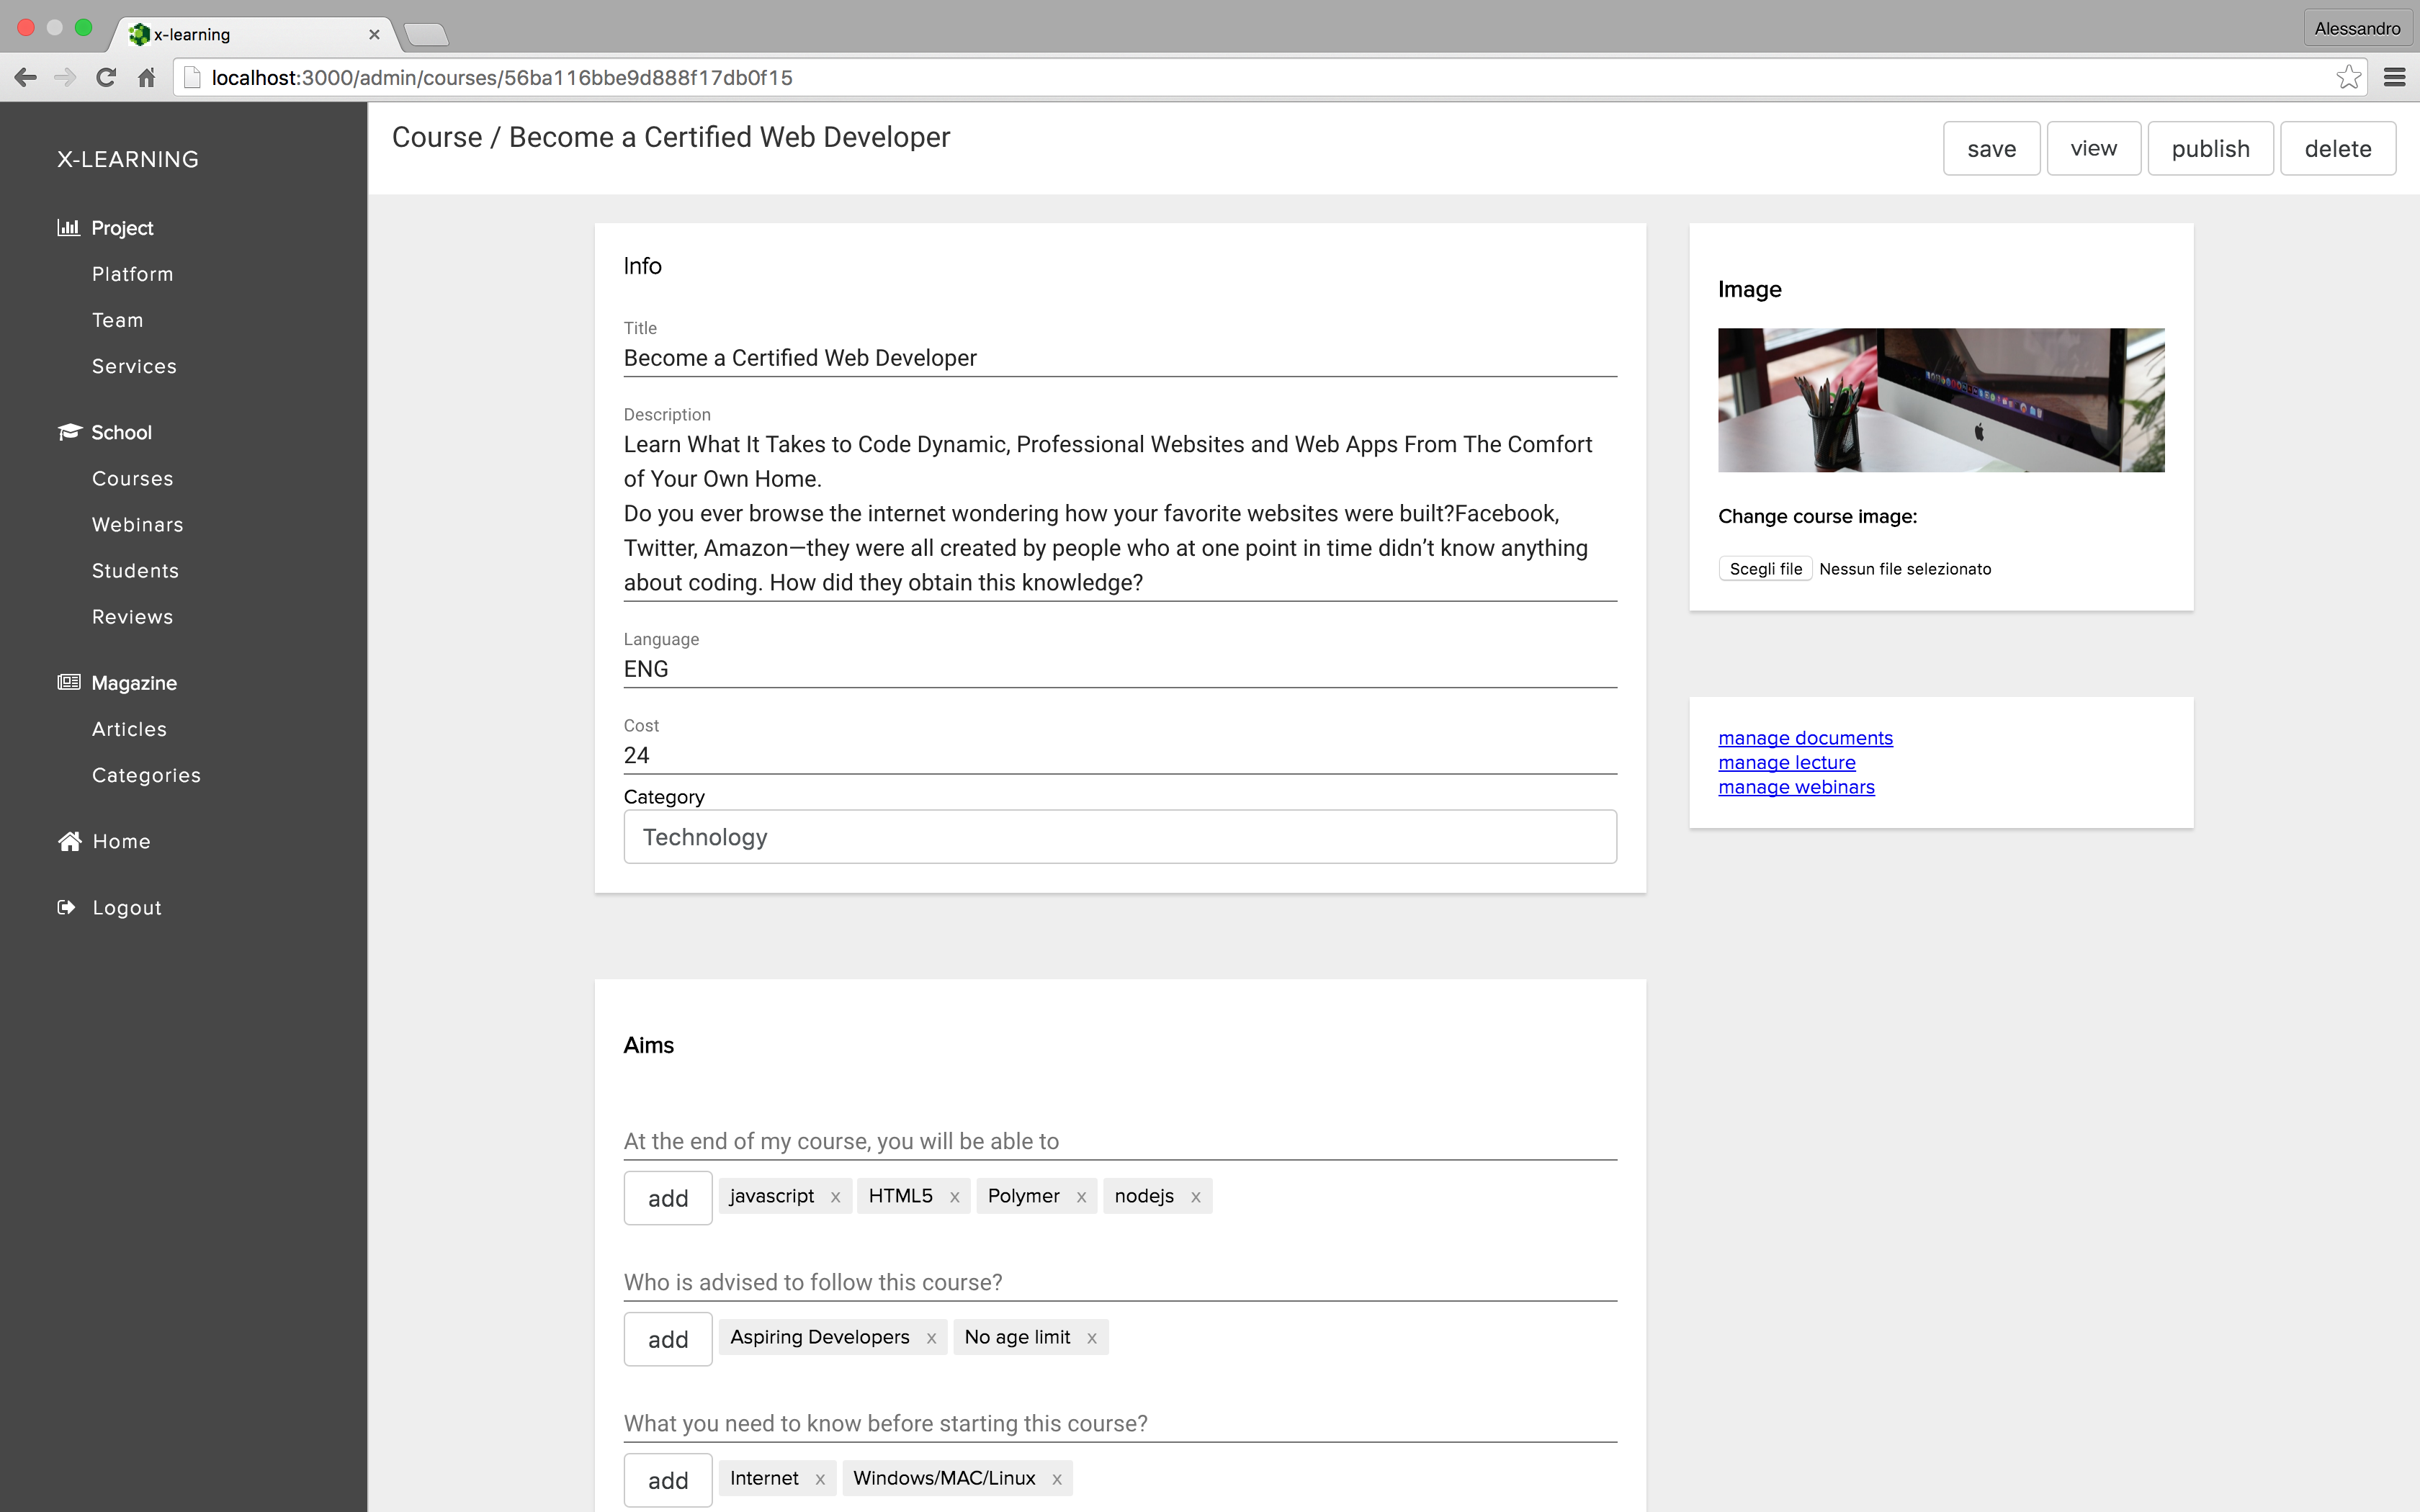
\includegraphics[width=1.0\linewidth]{images/chapter4/page-course-admin.png}
    \captionof{figure}[page course admin]{page course admin}
\end{minipage}

\item \textbf{page lecture} L'immagine seguente rappresenta la page lecture dove il teacher può gestire la creazione e la modifica di tutte le informazioni della singola lecture\par

\begin{minipage}{\linewidth}
    \centering
    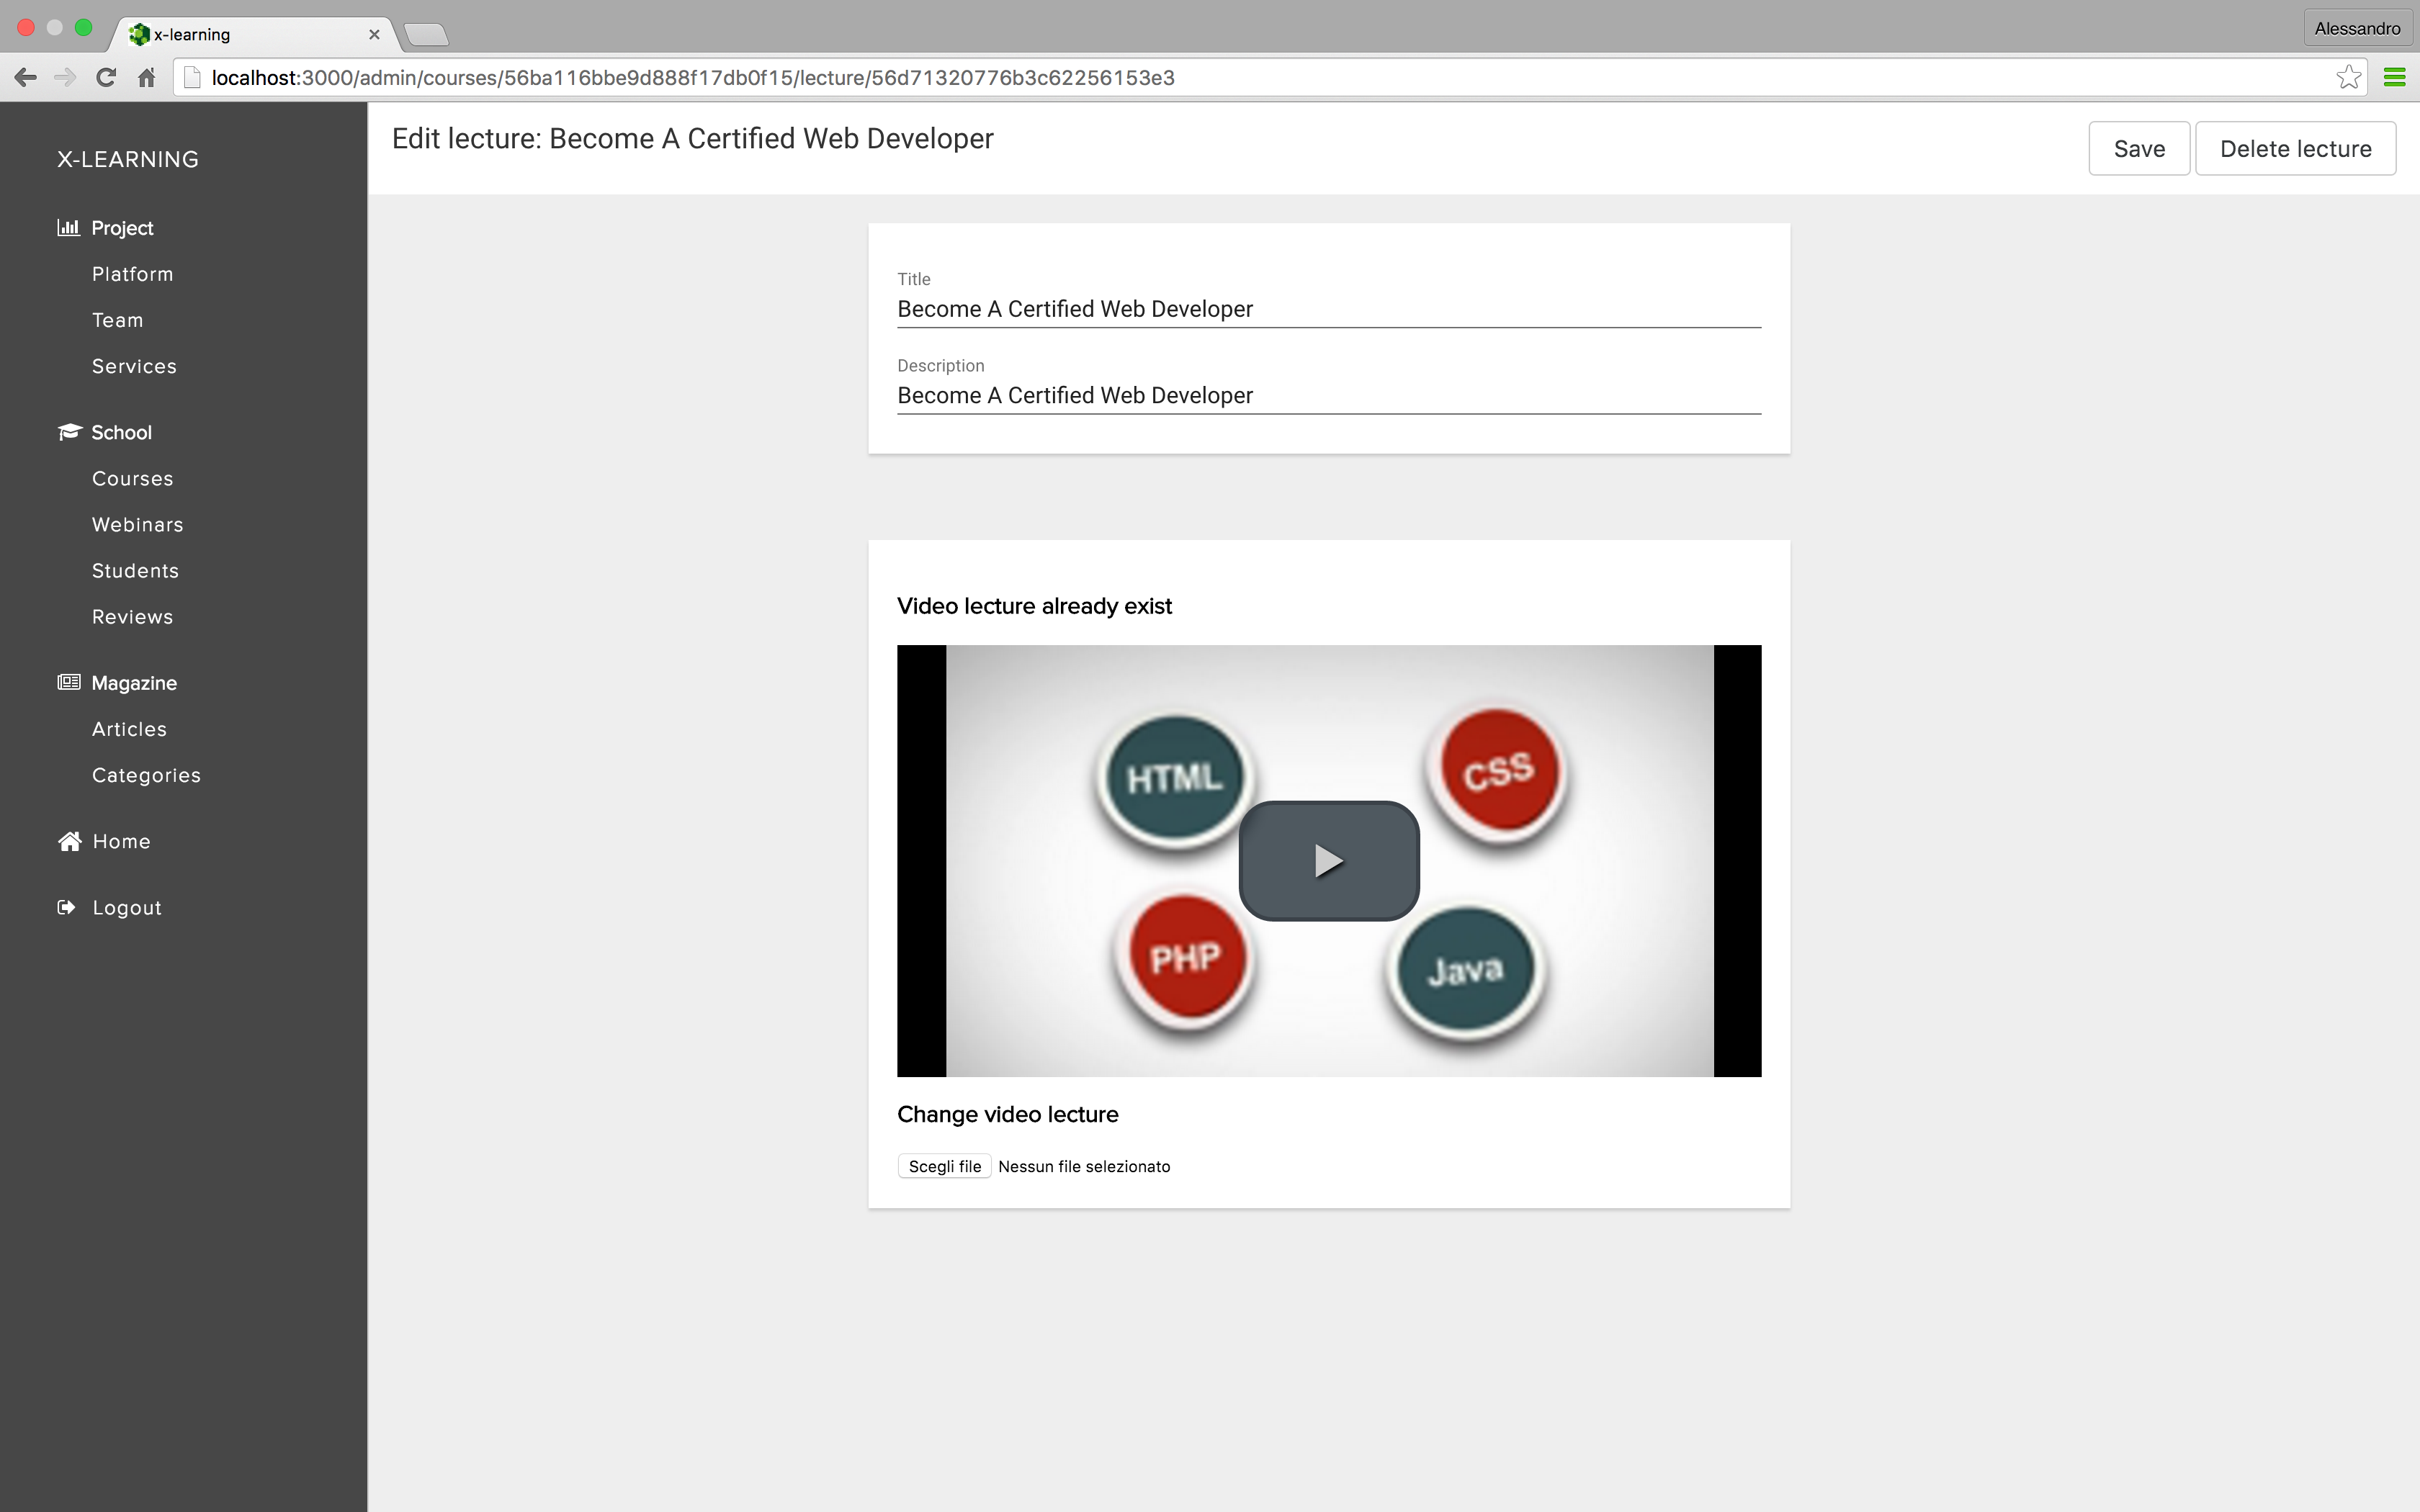
\includegraphics[width=1.0\linewidth]{images/chapter4/page-lecture-admin.png}
    \captionof{figure}[page lecture admin]{page lecture admin}
\end{minipage}

\item \textbf{page webinar} L'immagine seguente rappresenta la page lecture dove il teacher può gestire la creazione e la modifica di tutte le informazioni di un singolo webinar\par

\begin{minipage}{\linewidth}
    \centering
    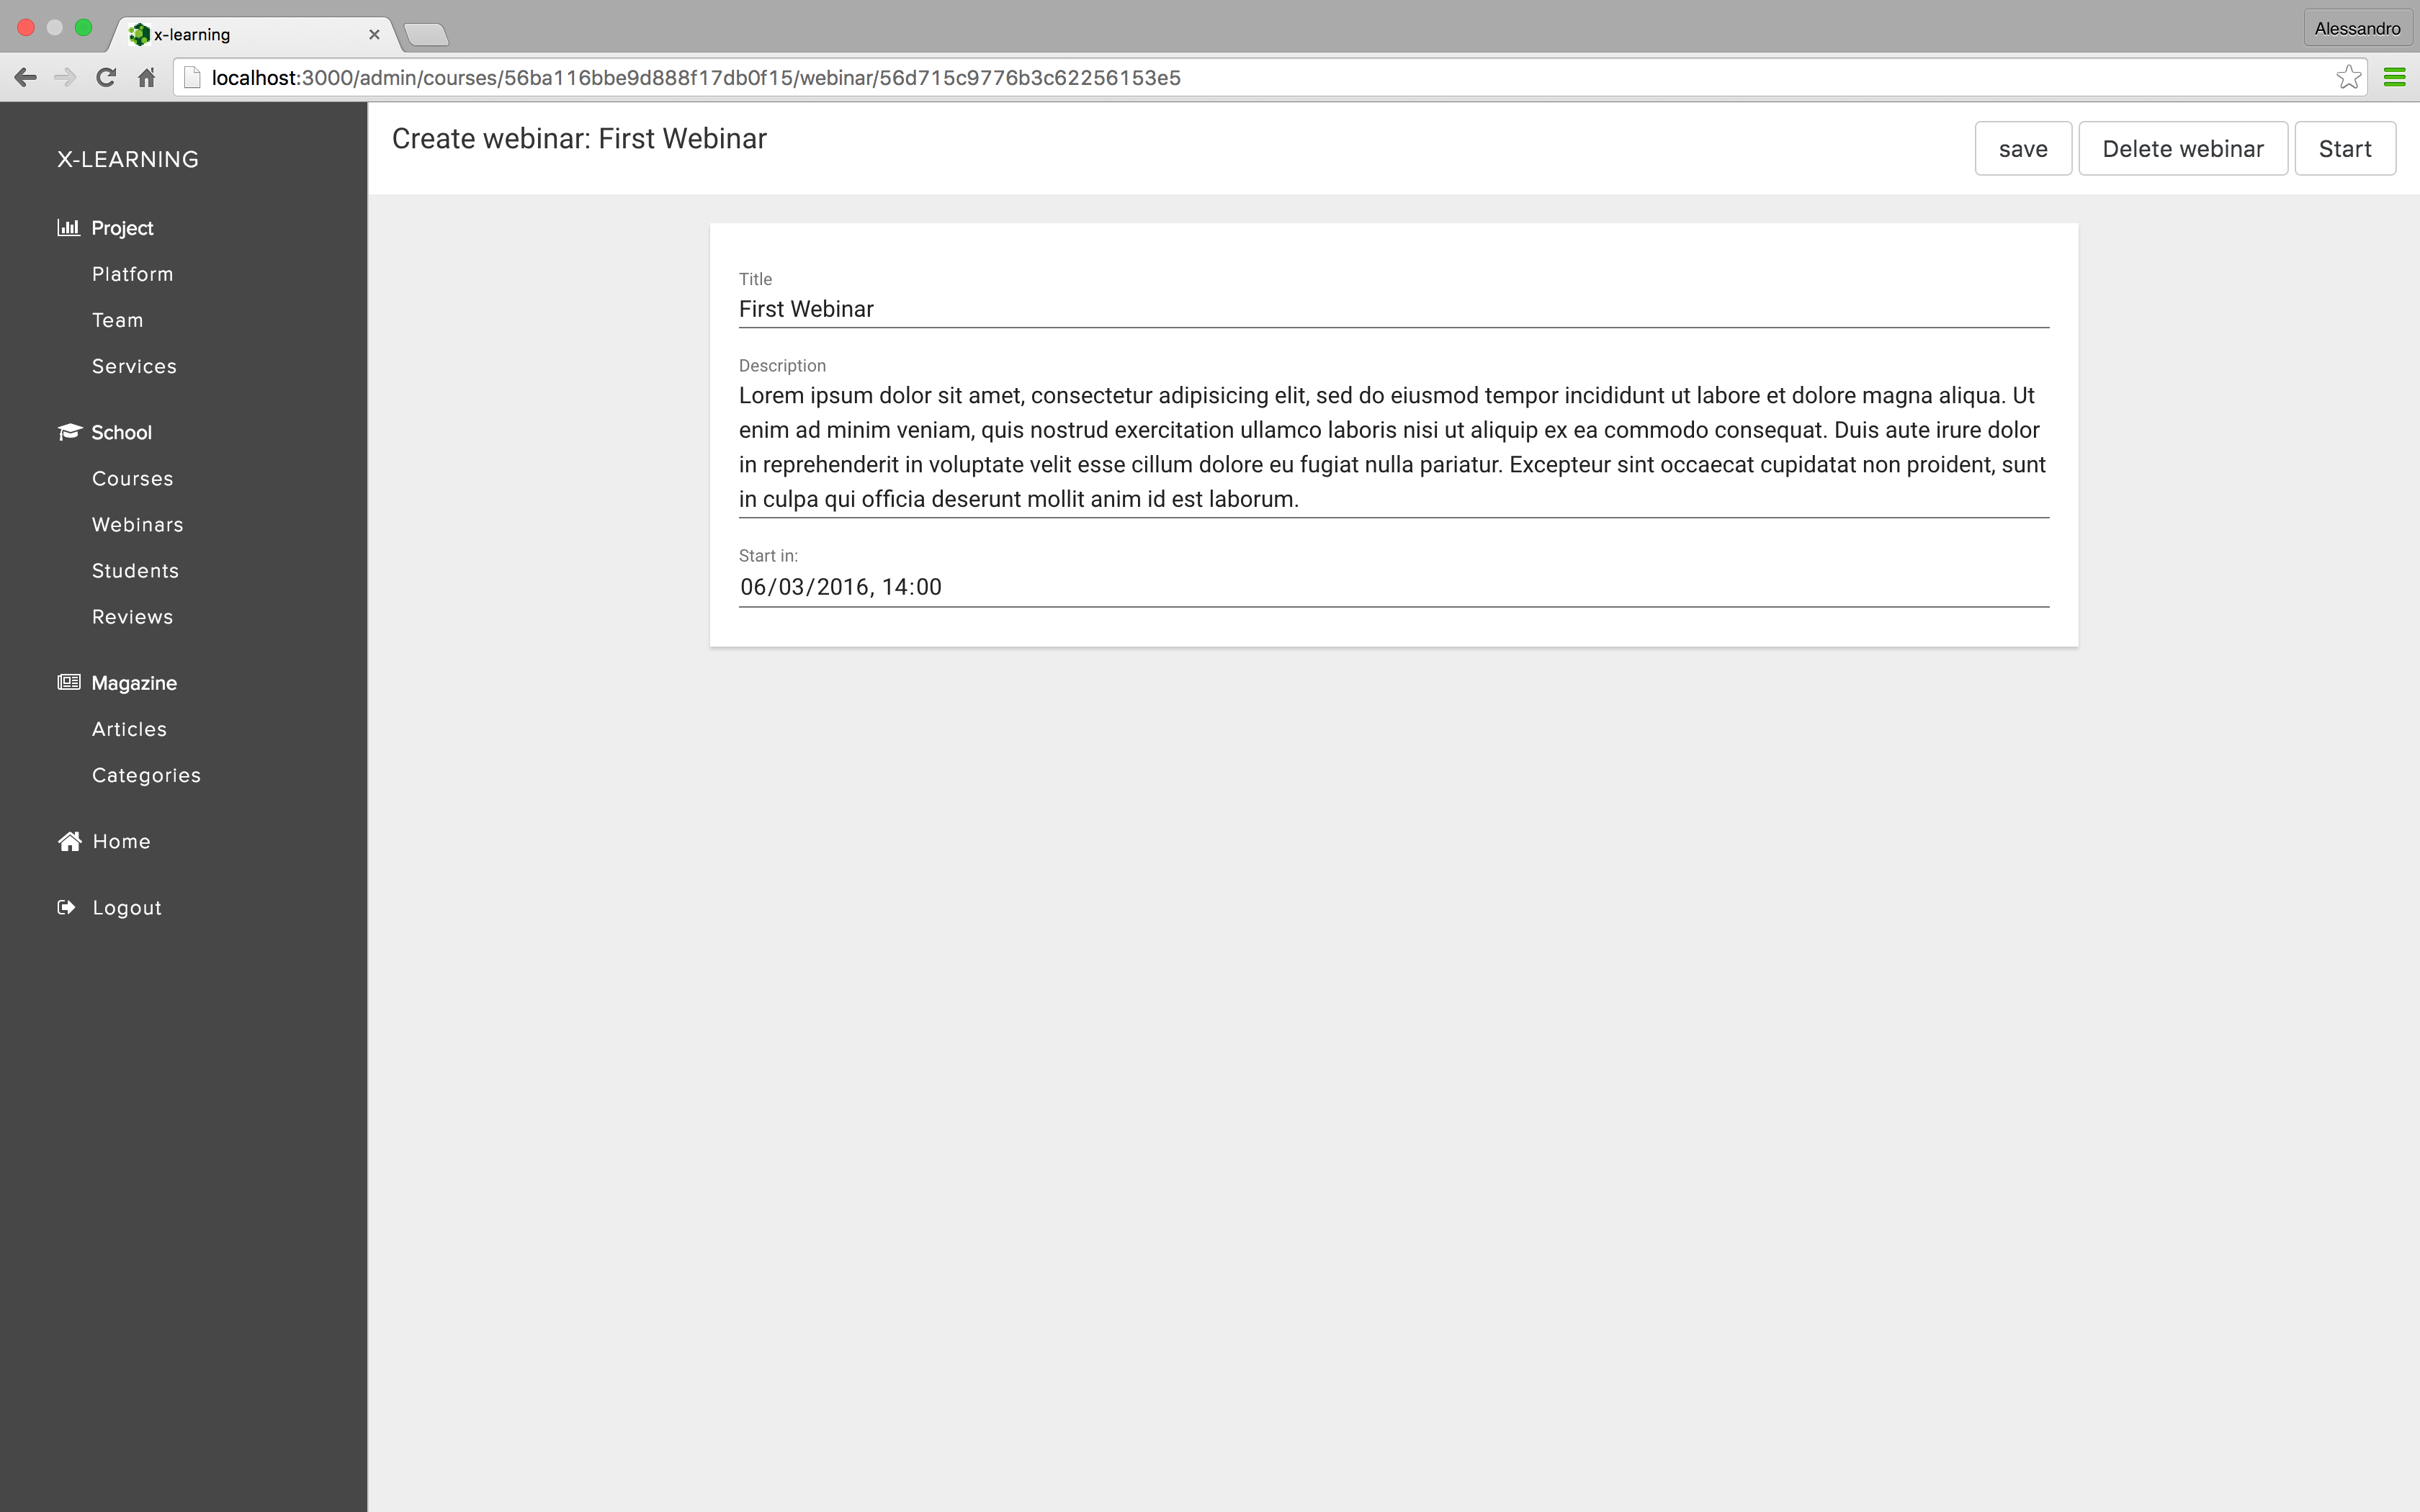
\includegraphics[width=1.0\linewidth]{images/chapter4/page-webinar-admin.png}
    \captionof{figure}[page webinar admin]{page webinar admin}
\end{minipage}

\end{itemize}


\subsubsection {Client side}
\label{subsec:Client_side}
The client side is the part of the platform that allows users to view courses and then attend lectures, webinars and access to educational materials.
The main pages that compose the client side are:

\begin{itemize}

\item \textbf{page home} L'immagine seguente rappresenta la Page Home dove lo student può cercare un determinato corso, vedere quelli disponibili, e eventualmente filtrari per categoria\par

\begin{minipage}{\linewidth}
    \centering
    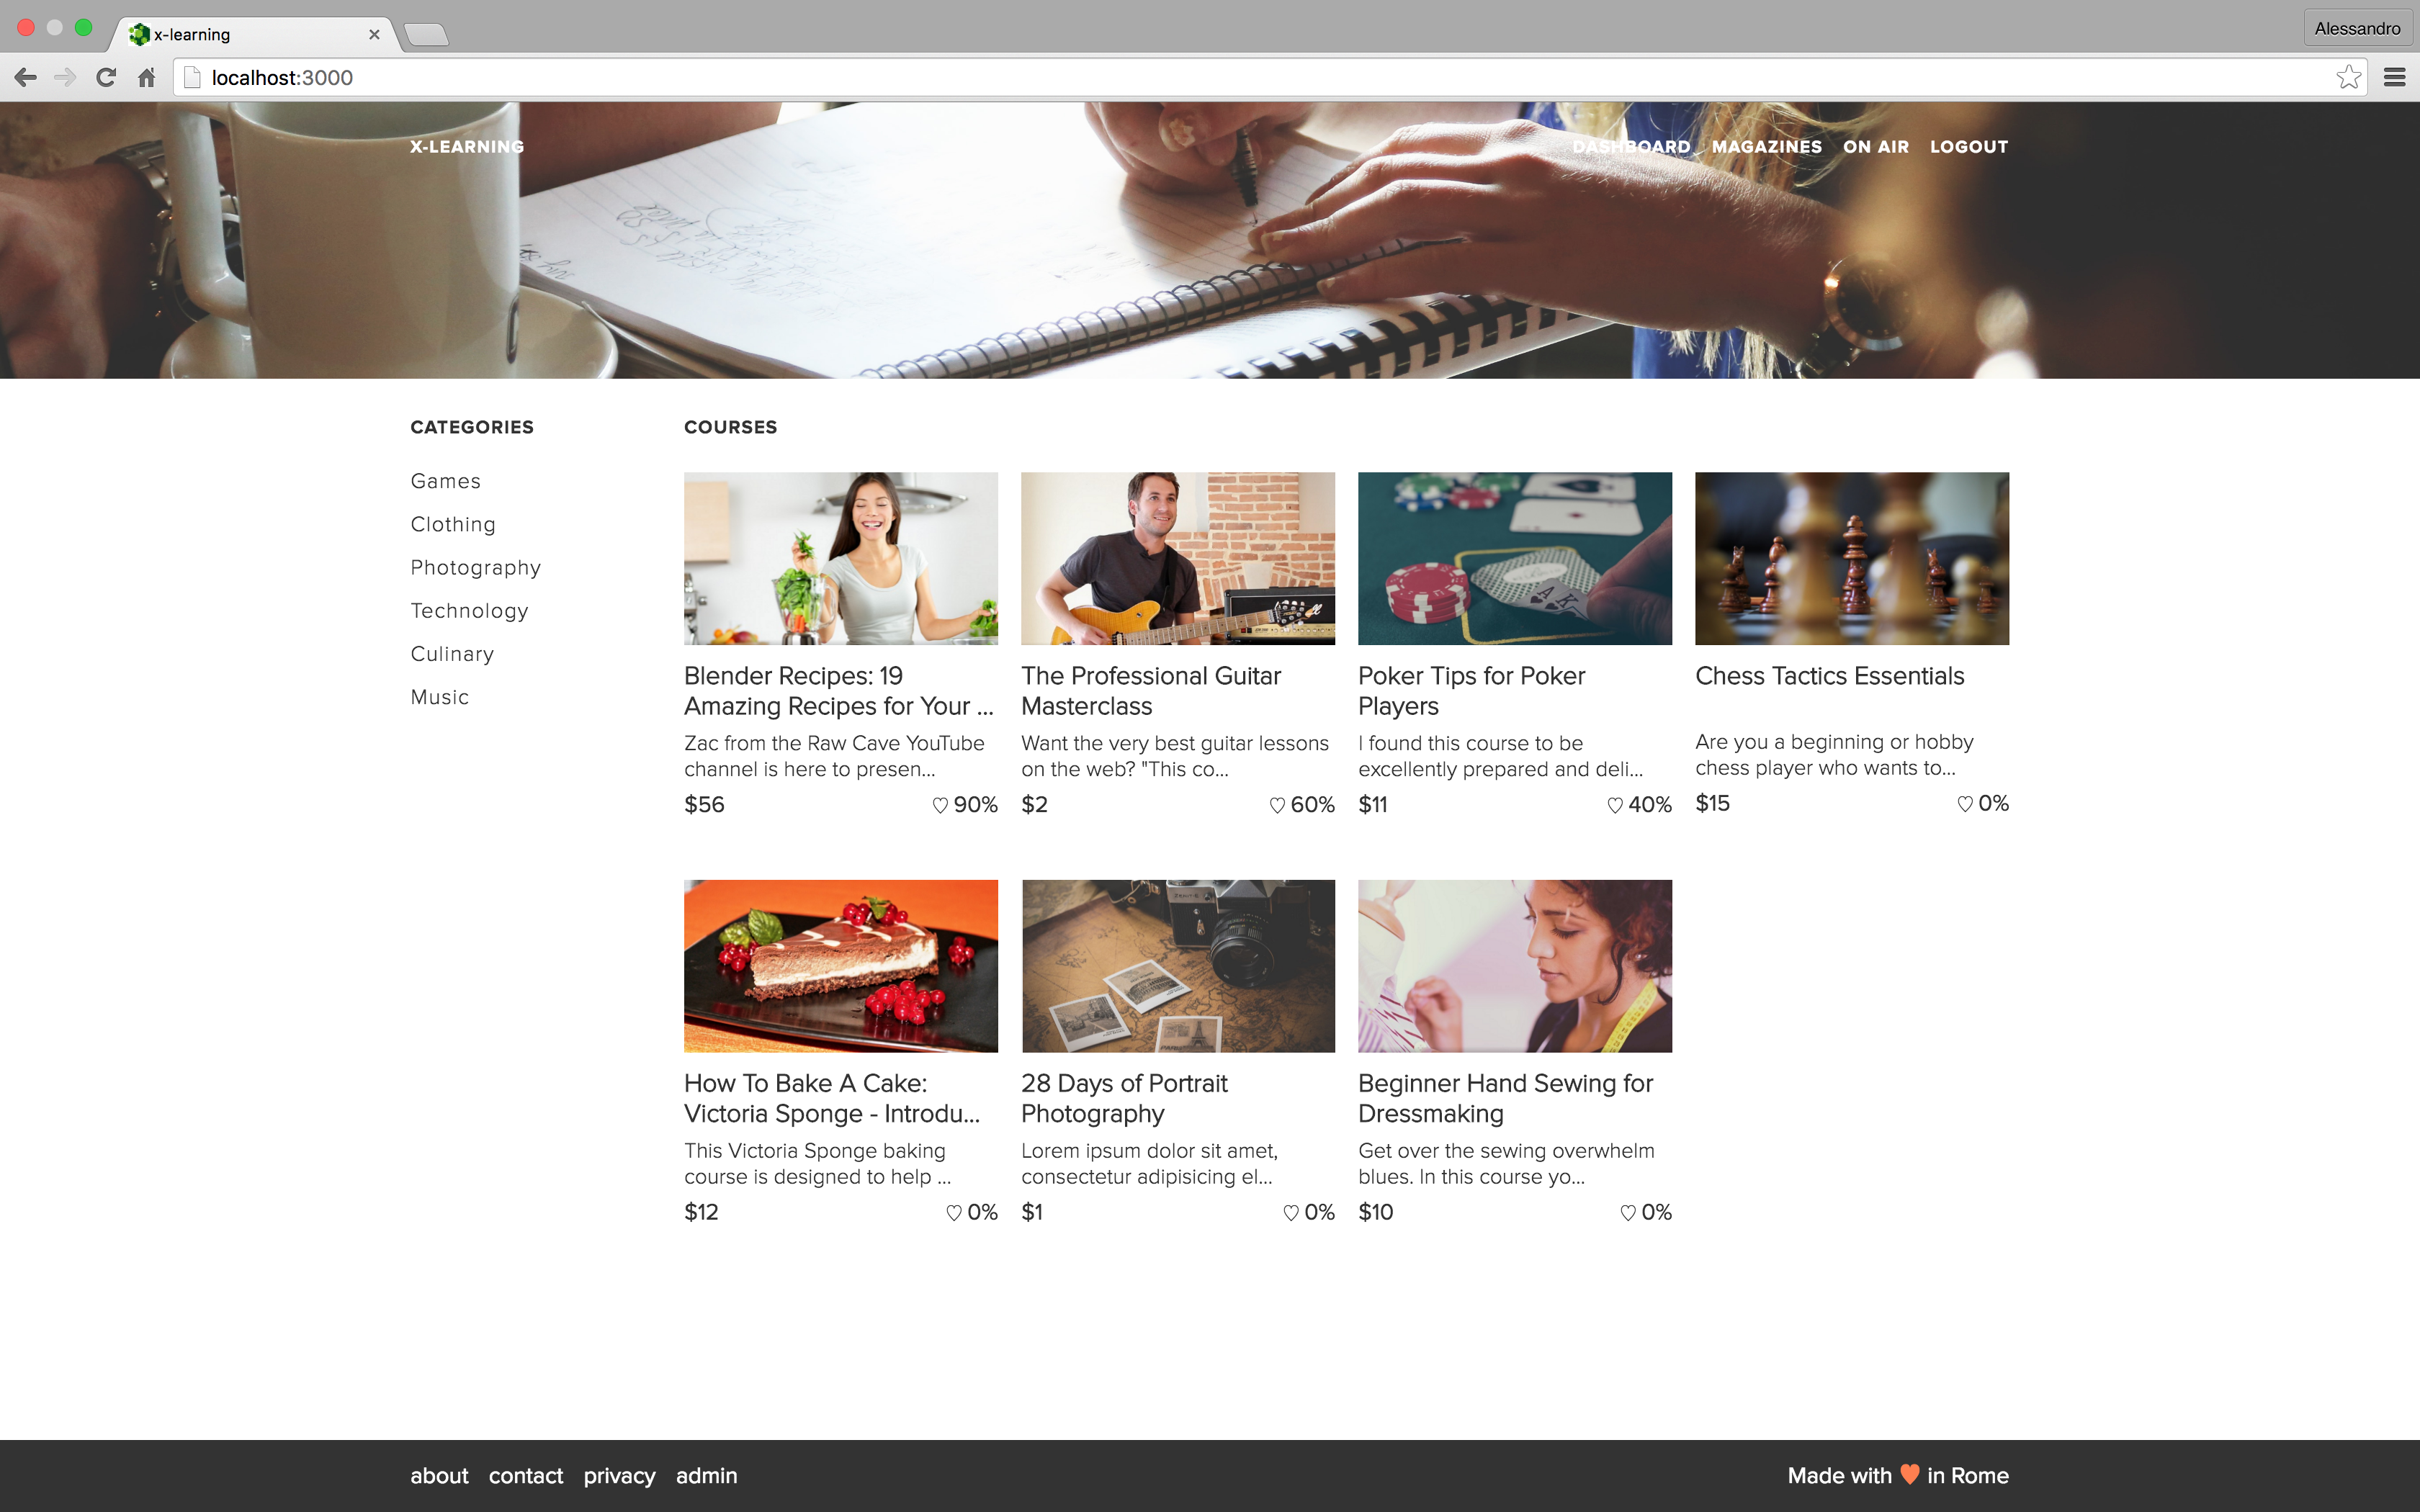
\includegraphics[width=1.0\linewidth]{images/chapter4/page-home.png}
    \captionof{figure}[page home]{page home}
\end{minipage}


\item \textbf{page course} L'immagine seguente rappresenta la Page Course dove è possibile trovare tutte le informazioni di un singolo corso come costo, review, video lezioni, materiale didattico \par
\begin{minipage}{\linewidth}
    \centering
    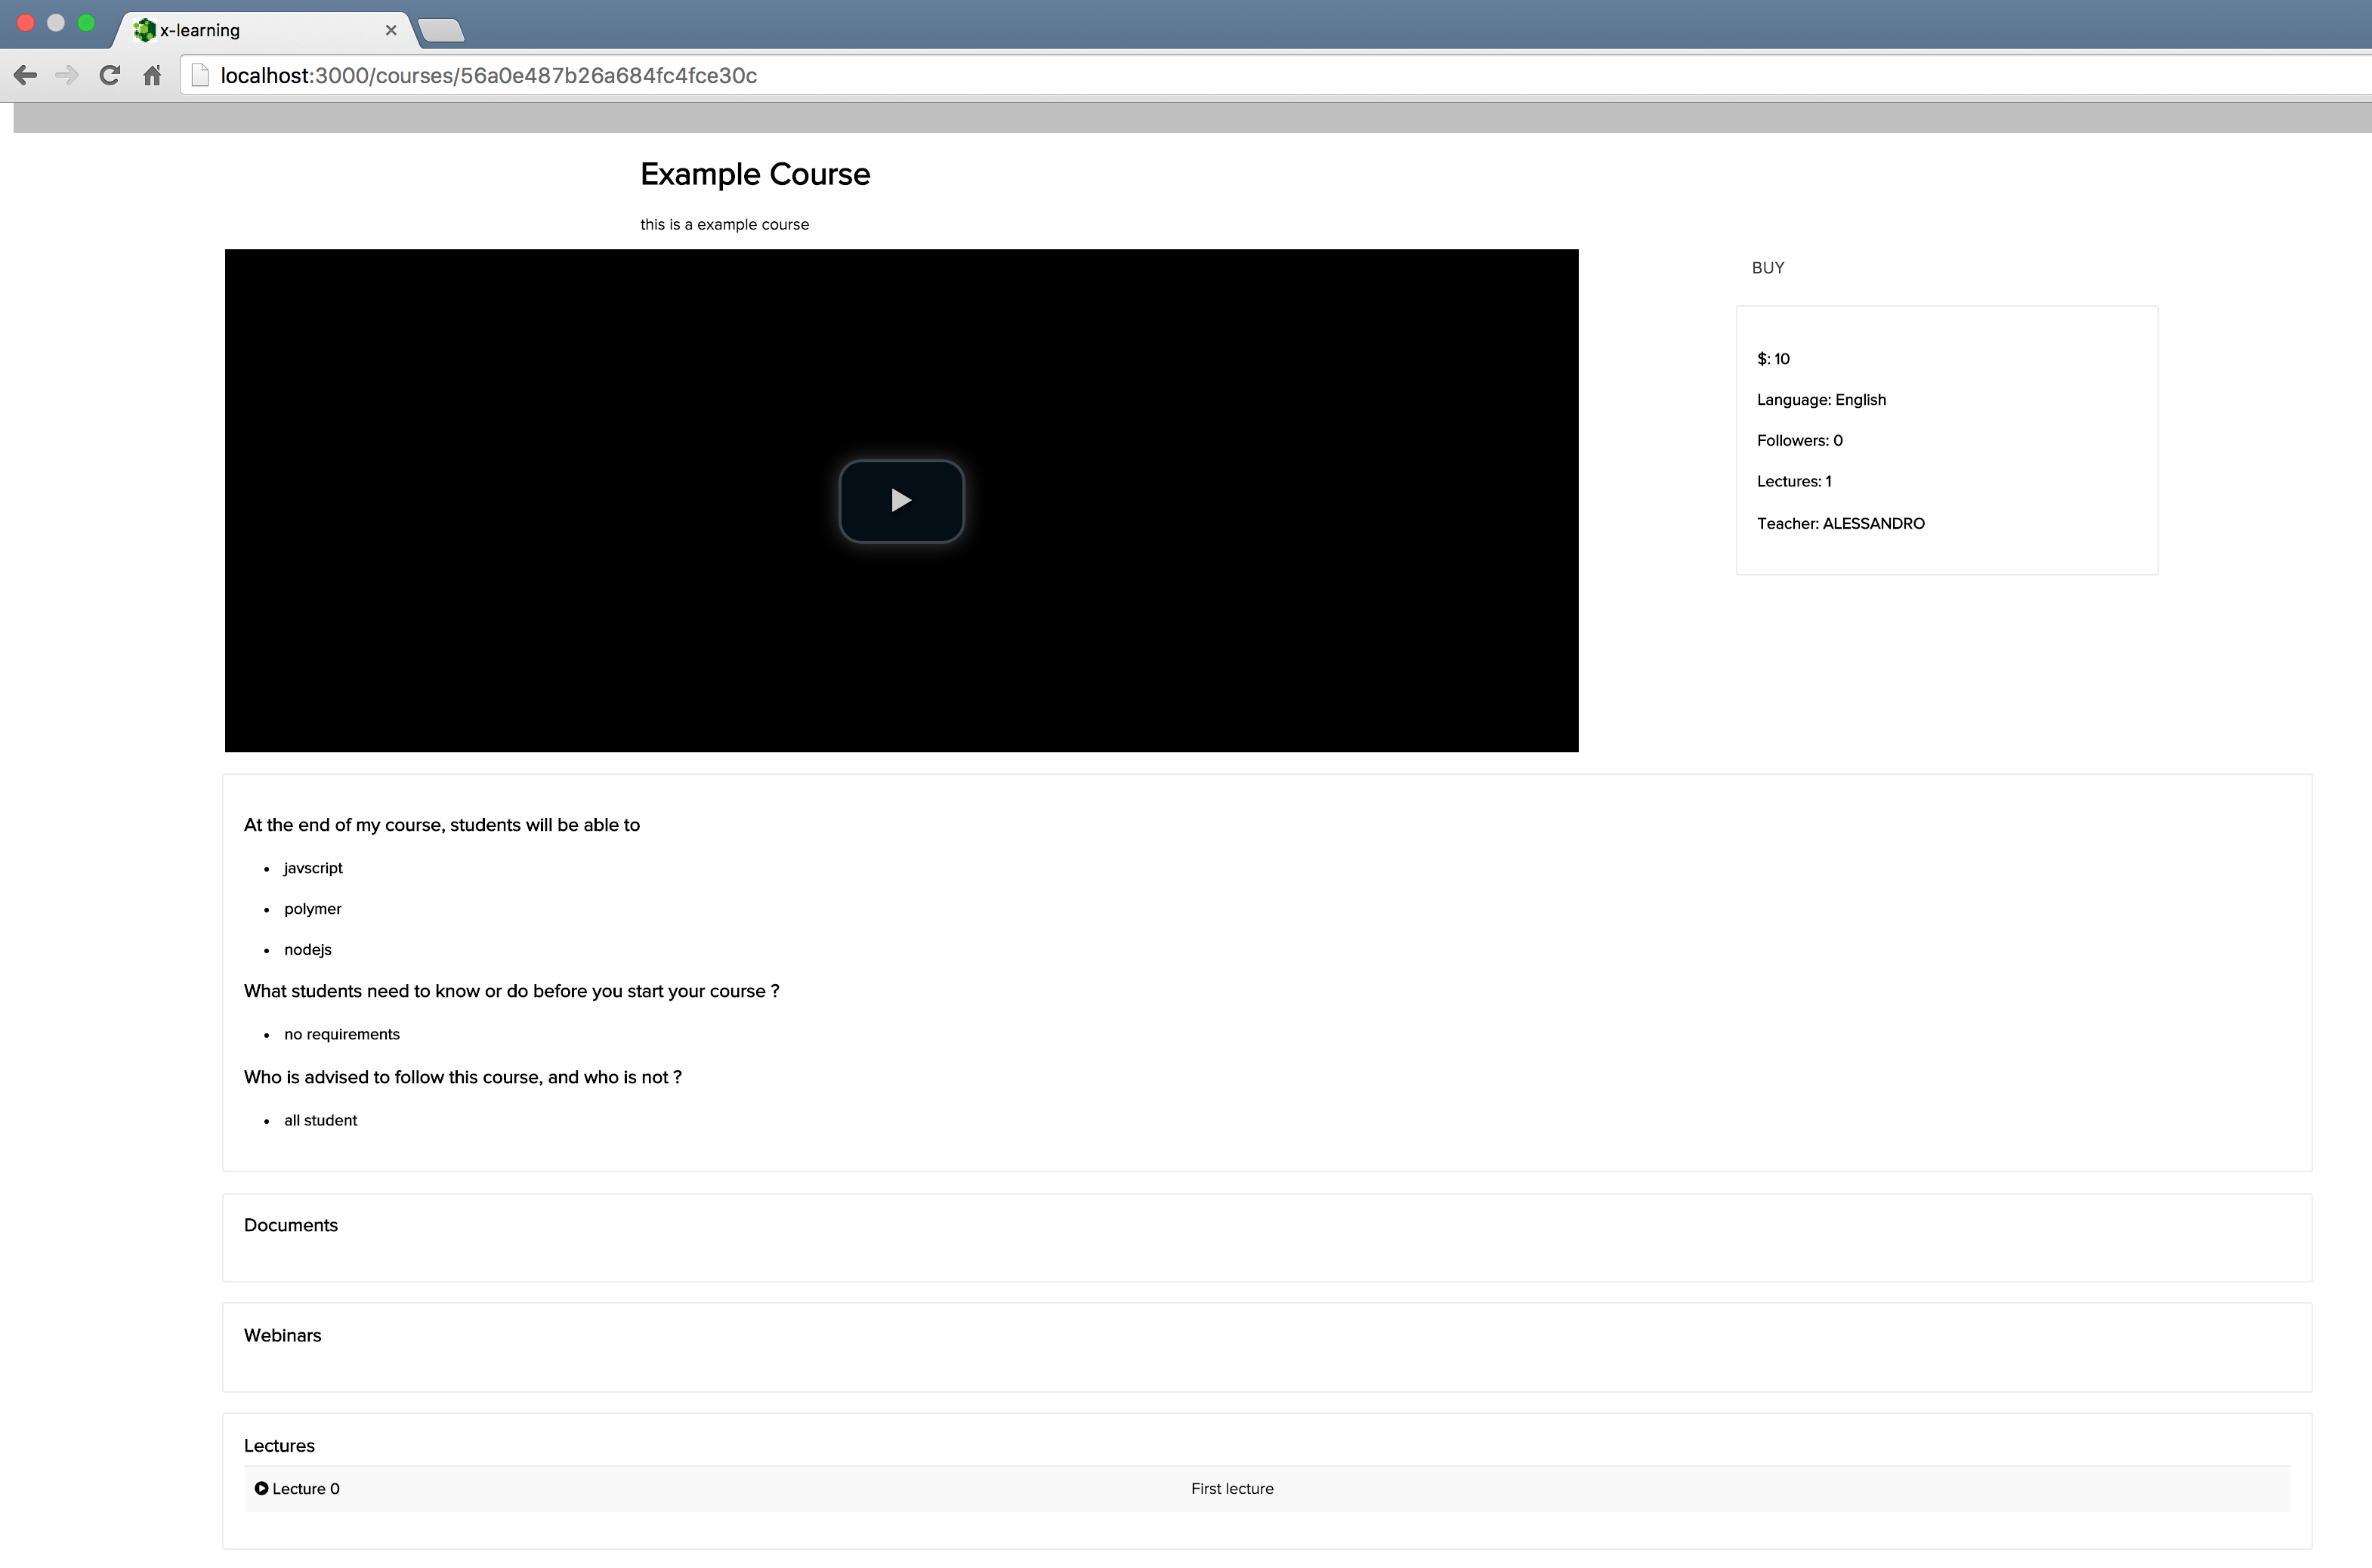
\includegraphics[width=1.0\linewidth]{images/chapter4/page-course.png}
    \captionof{figure}[page course]{page course}
\end{minipage}


\item \textbf{page lecture} L'immagine seguente rappresenta la Page lecture che permette la visualizzazione della video lezione\par

\begin{minipage}{\linewidth}
    \centering
    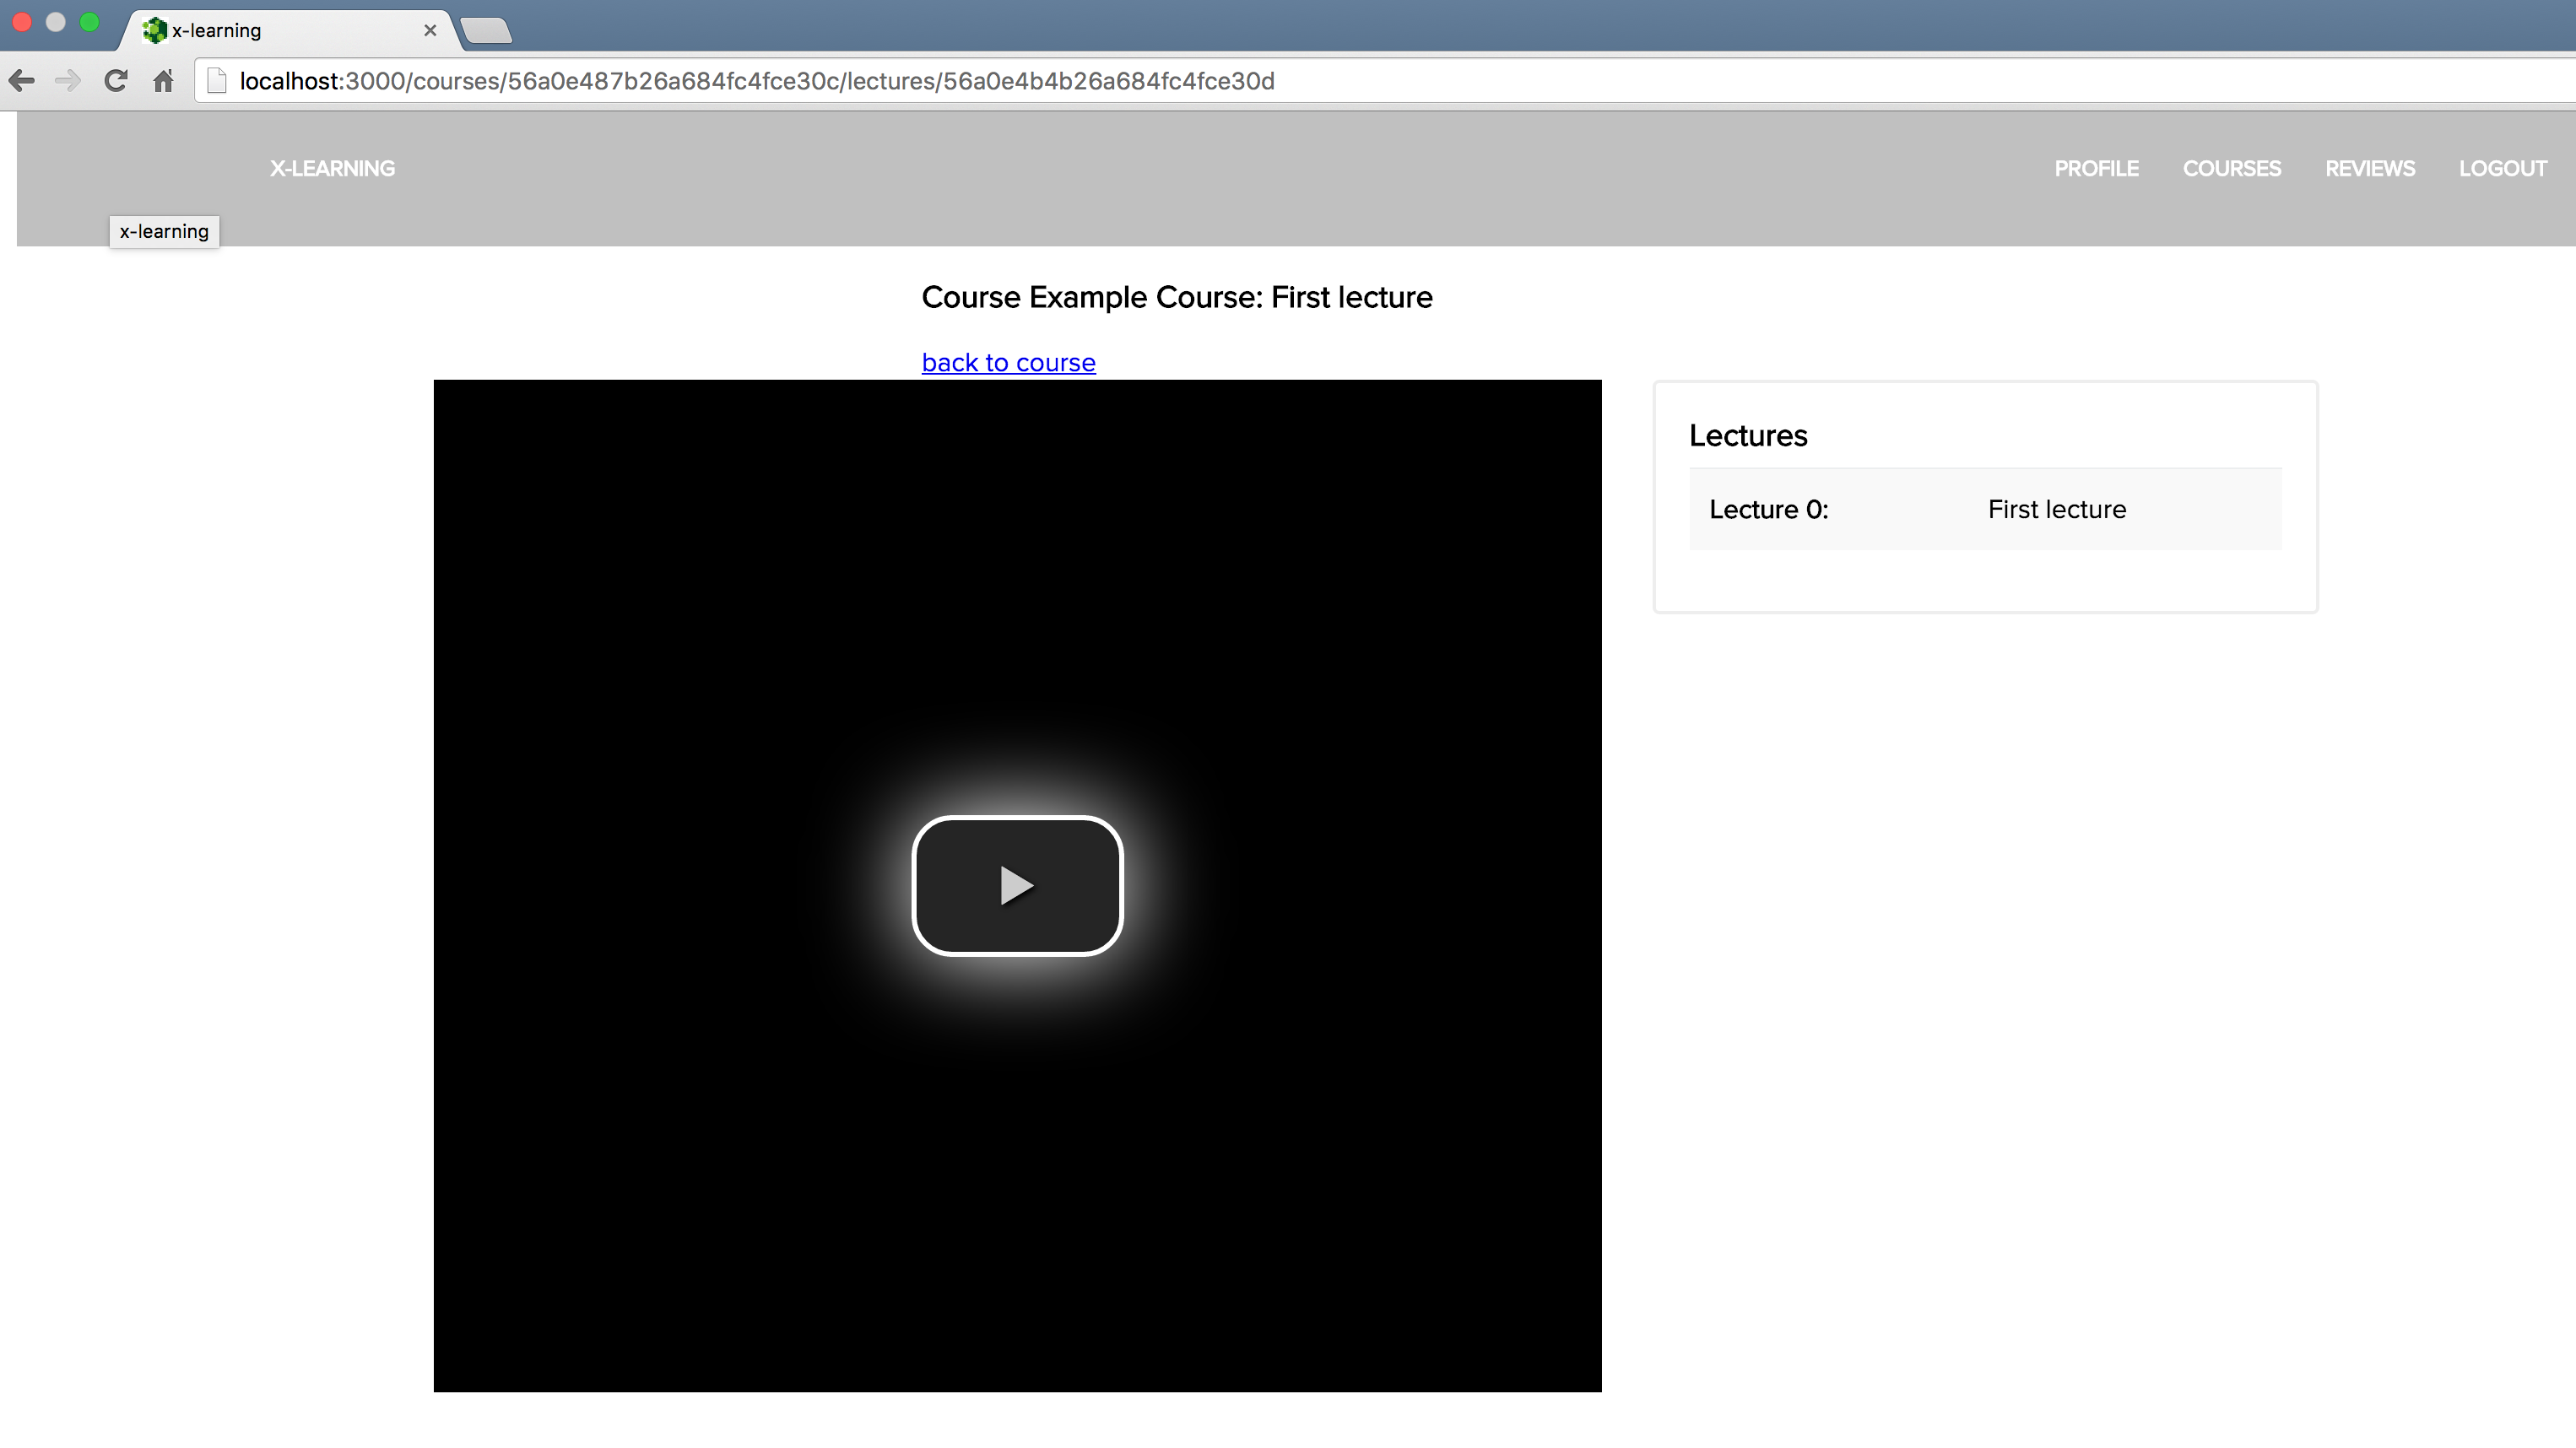
\includegraphics[width=1.0\linewidth]{images/chapter4/page-lecture.png}
    \captionof{figure}[page lecture]{page lecture}
\end{minipage}


\item \textbf{page webinar} L'immagine seguente rappresenta la Page Webinar che permette di collegarsi in tempo reale al webinar di un determianto corso\par
\begin{minipage}{\linewidth}
    \centering
    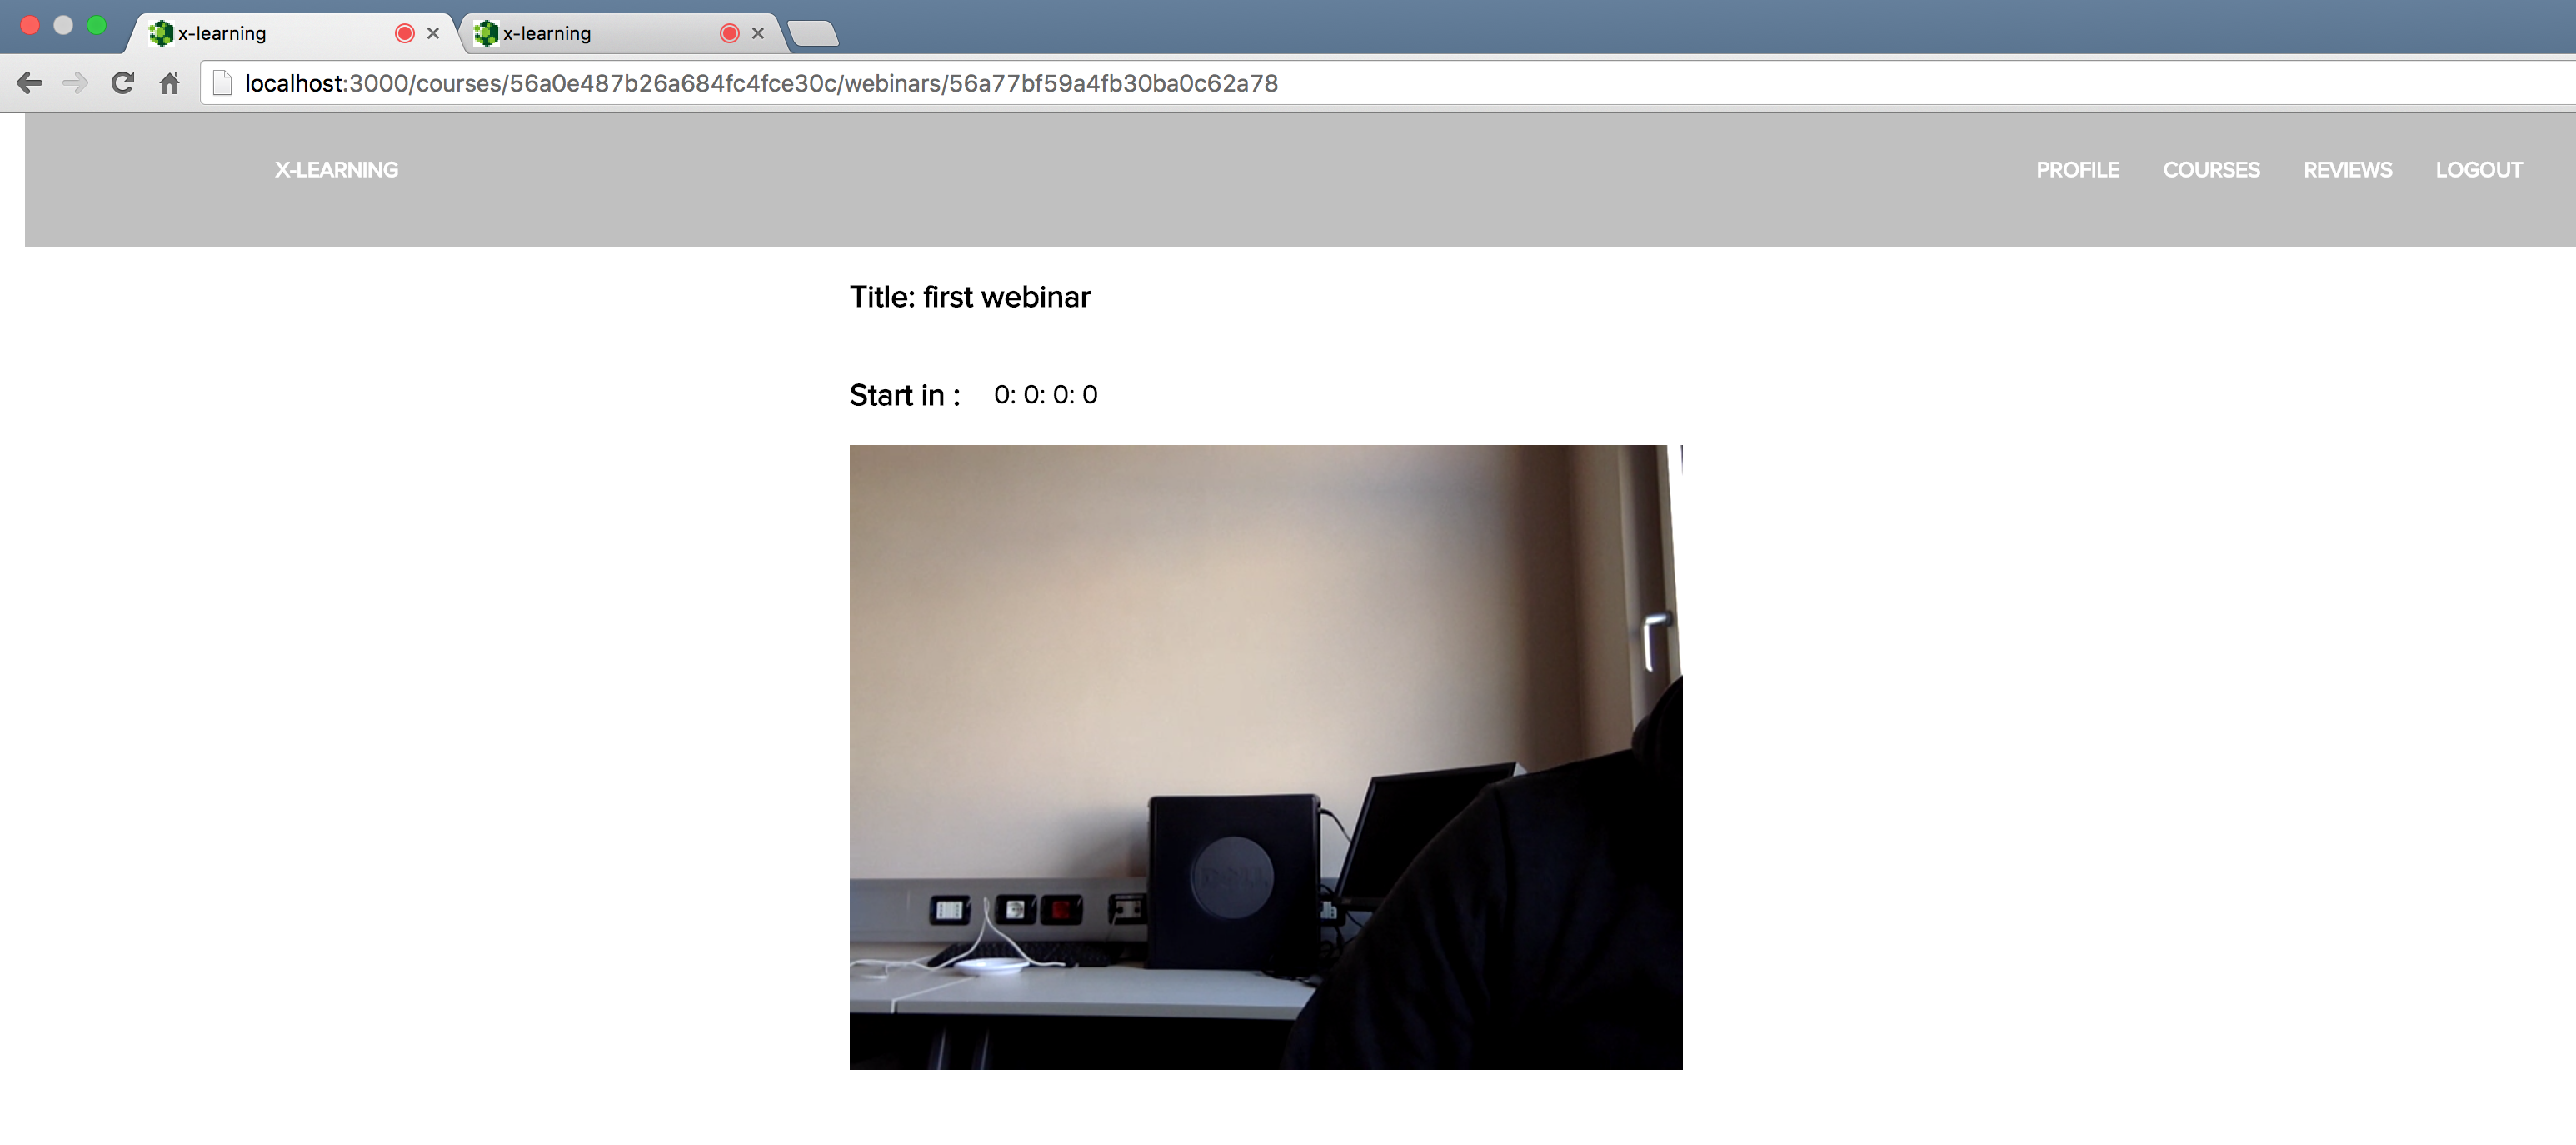
\includegraphics[width=1.0\linewidth]{images/chapter4/page-webinar.png}
    \captionof{figure}[page webinar]{page webinar}
\end{minipage}

\end{itemize}



\subsubsection { UI components assembly}
\label{subsec:4th_step_UI_components_assembly}

Distinct UI components are finally mounted to compose the application views. Assembly is kept as simple as possible: it only consists of a composition of HTML5 elements. So, the entire development process results driven by: JSON documents describing entities of the application and HTML template documents describing the UI components.
{\color{red} The following is an example: }

\begin{figure}[htb] %  figure placement: here, top, bottom
 \centering
 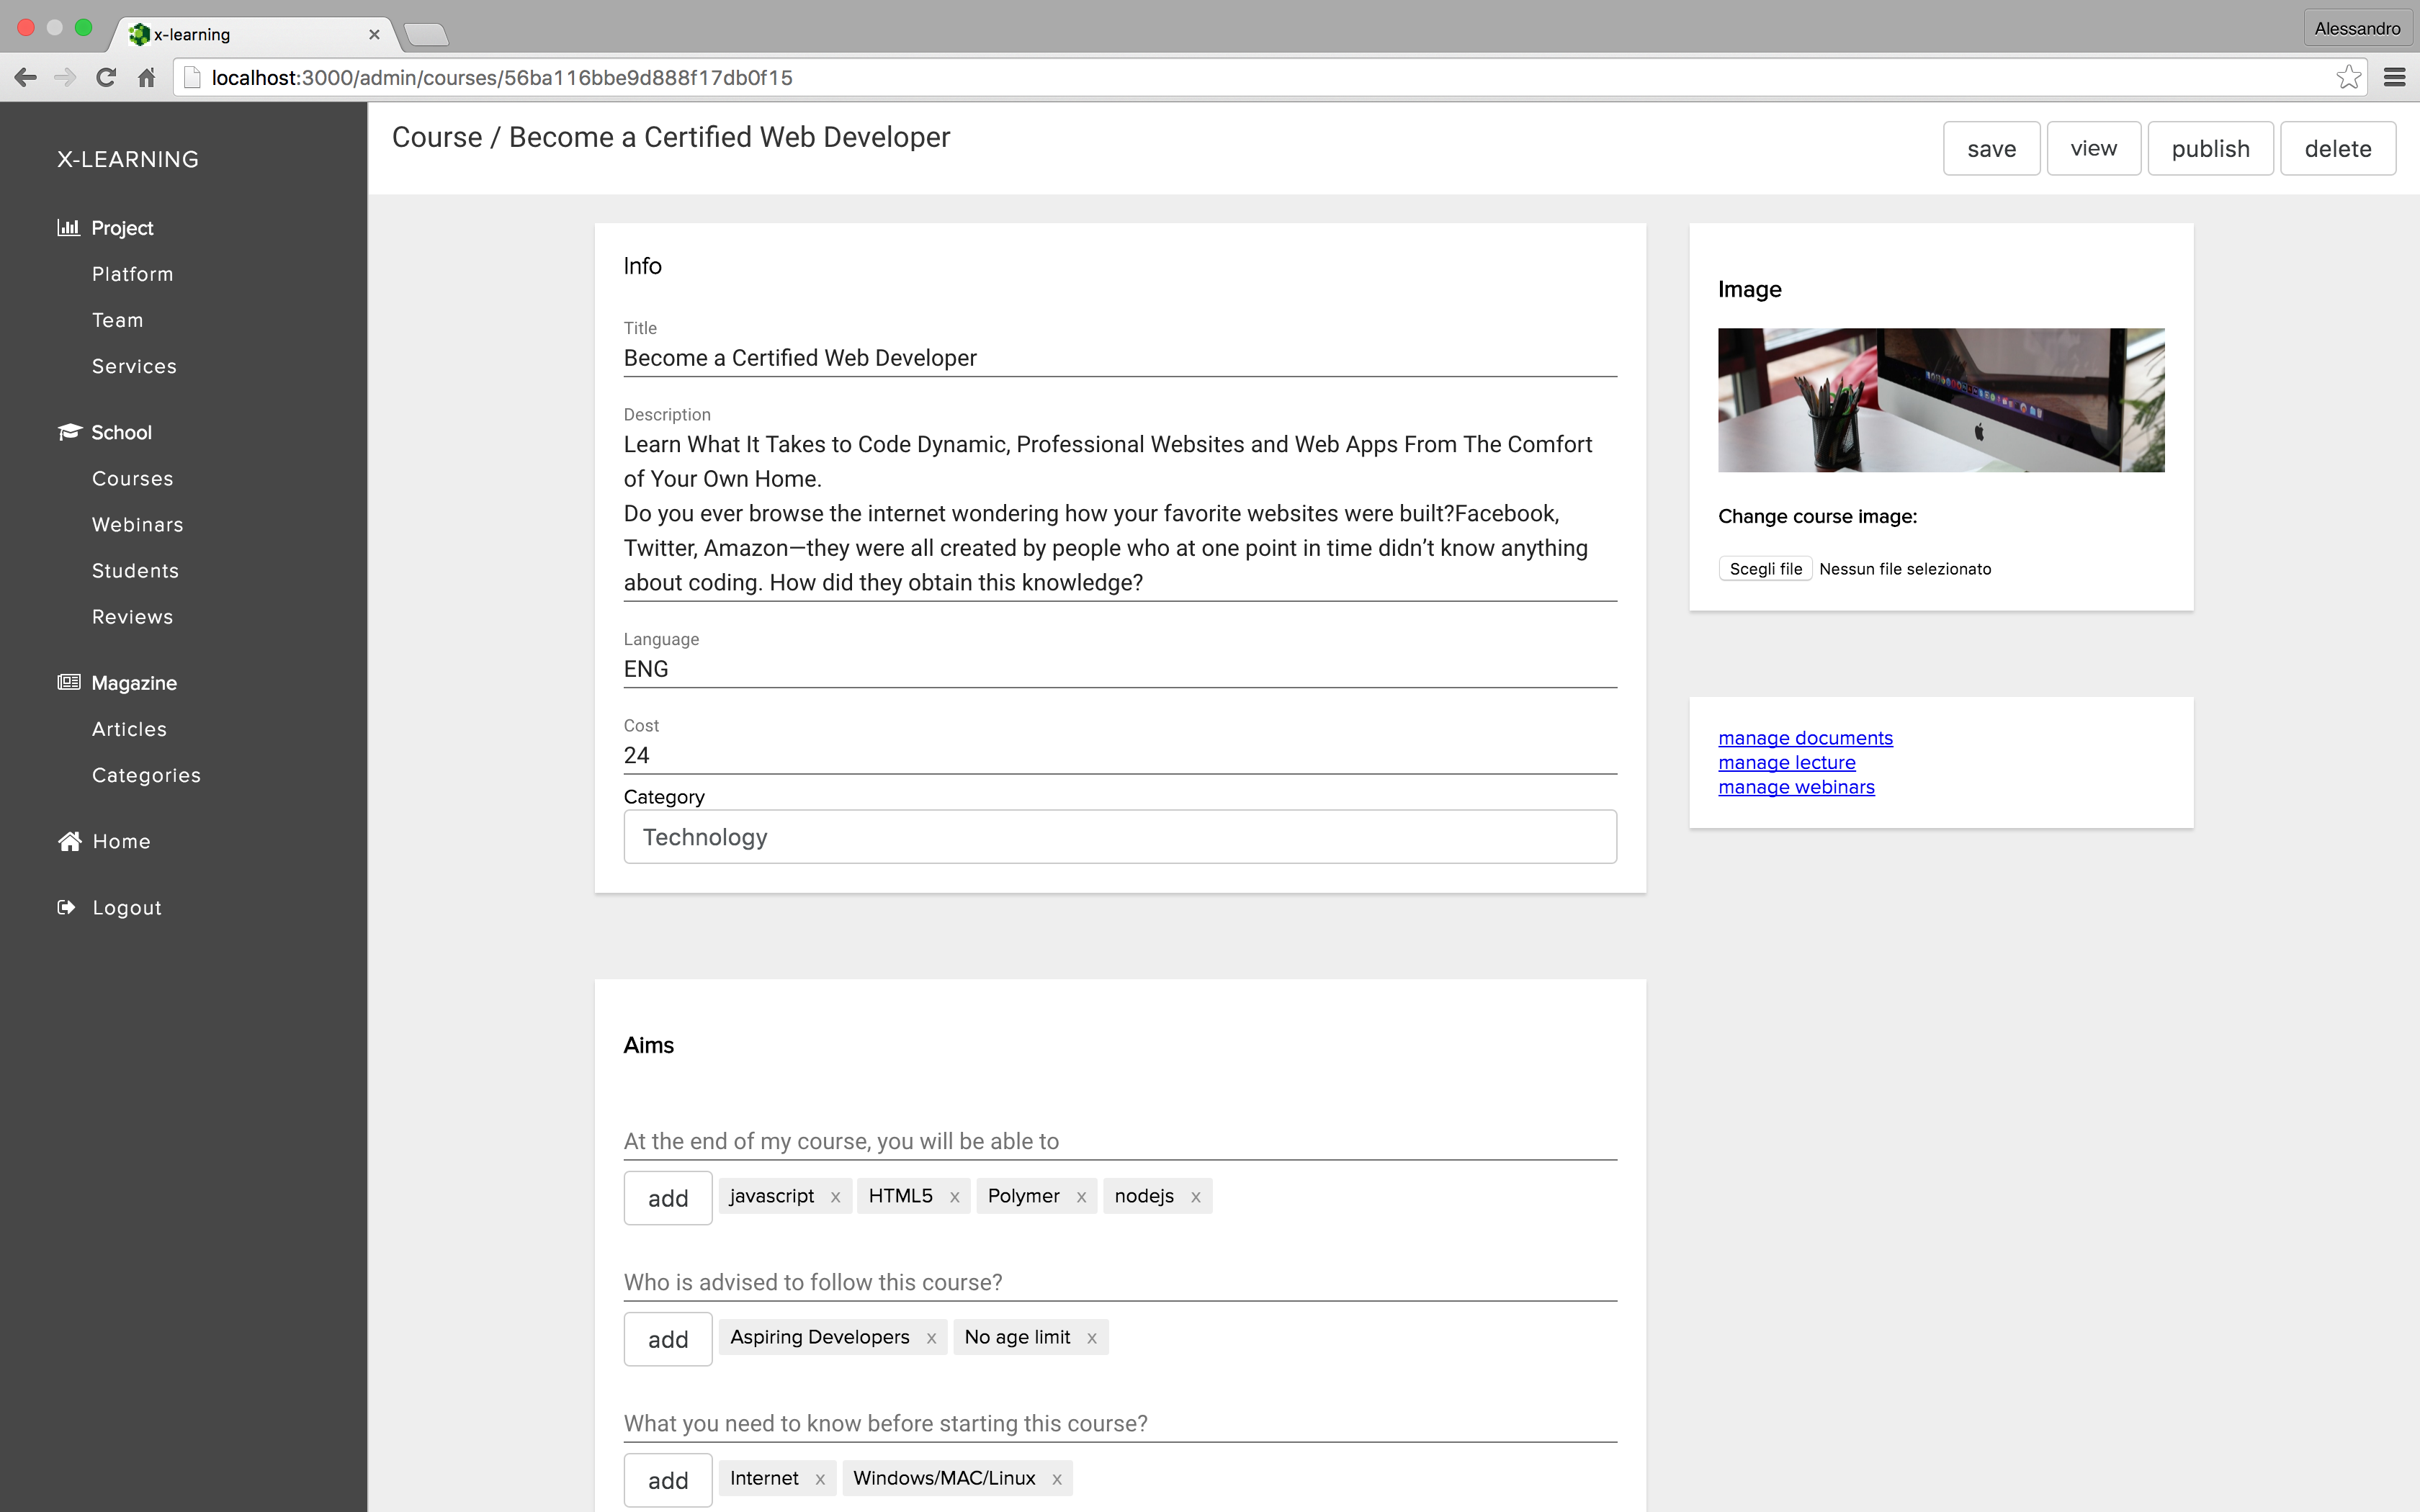
\includegraphics[width=1.0\linewidth]{images/chapter4/page-course-admin.png}\hfill
 \caption[Page Admin course action]{Page Admin course action}
 \label{fig:fourV}
\end{figure}

In the image below shows the edit page of the course composed of the following Web component:

\begin{lstlisting}[language=html]
<part-course-actions course="{{course}}"></part-course-actions>
\end{lstlisting}


\begin{figure}[htb] %  figure placement: here, top, bottom
 \centering
 
\includegraphics[width=1.0\linewidth]{images/chapter4/admin-course-actions.png}\hfill
 \caption[Page Admin course action]{Page Admin course action}
 \label{fig:fourV}
\end{figure}

\begin{lstlisting}[language=html]
<part-course-info course="{{course}}" error="{{error}}"></part-course-info>
\end{lstlisting}



\begin{minipage}{\linewidth}
    \centering
    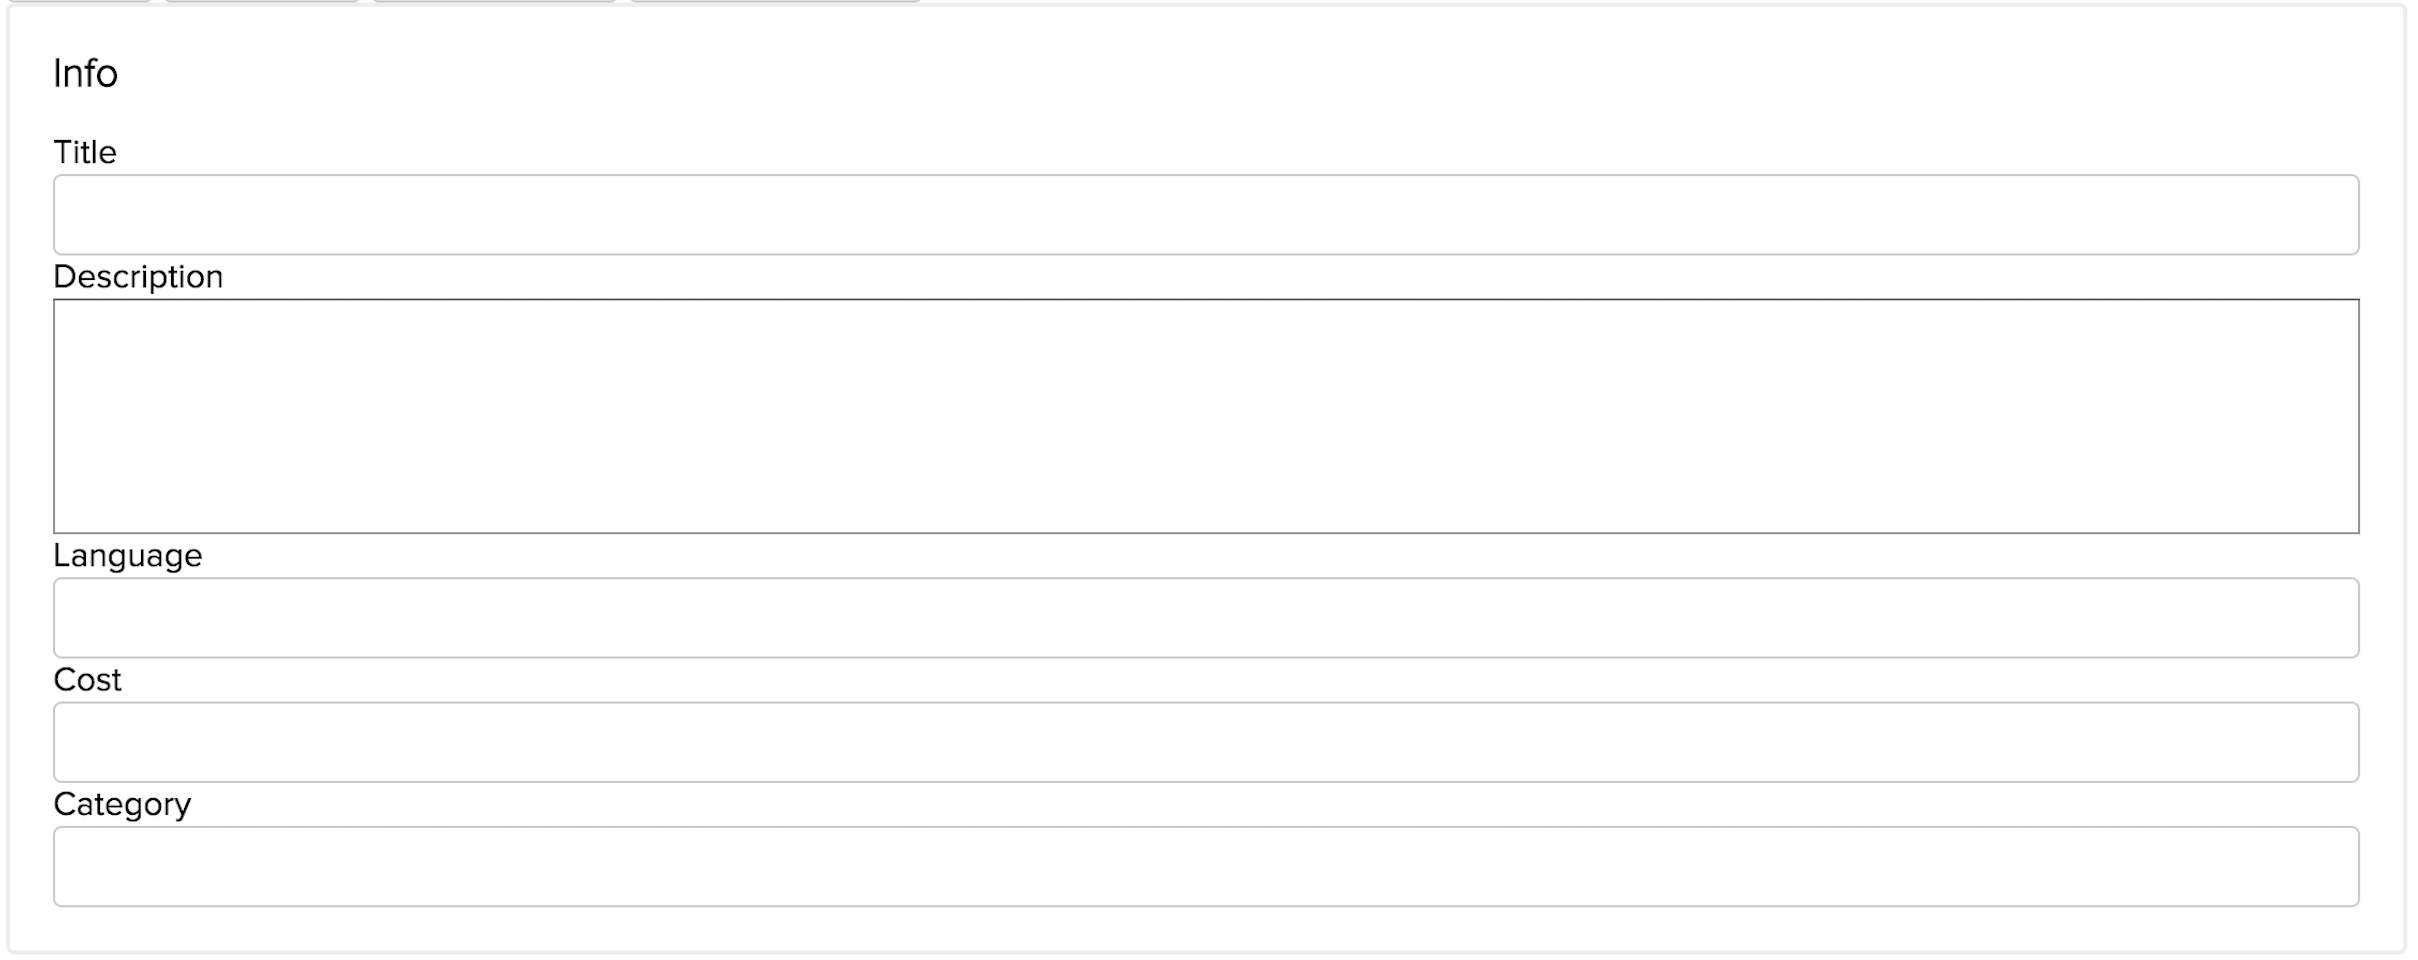
\includegraphics[width=1.0\linewidth]{images/chapter4/admin-course-info.png}
    \captionof{figure}[Page Admin course info]{Page Admin course info}
\end{minipage}

Also as you can see on the page is given the opportunity to manage the different components of the course:
\begin{itemize}

\item \textbf{Image section}\par
\begin{itemize}
  \item add the image of the course
  \item change the image of the course
\end{itemize}

\item \textbf{Aims section} permette di inserire:

\begin{itemize}
  \item At the end of my course, students will be able to
  \item Who is advised to follow this course, and who is not ?
  \item What students need to know or do before you start your course ?
\end{itemize}

\item \textbf{Lectures section}\par 
\begin{itemize}
  \item manage the lessons of the course and so change and elimination
  \item link to the page for creating a new lesson that lets you enter information such as title description and upload the video  
\end{itemize}


\item \textbf{Webinar section}\par
\begin{itemize}
  \item manage the webinar of the course and so change and elimination
  \item link to the page for creating a new lesson that lets you enter information such as title description and set the date
\end{itemize}


\item \textbf{Document}\par
\begin{itemize}
  \item add documents to the course
  \item remove documents from the course
\end{itemize}

\end{itemize}




\section{Amazon SNS and SQS}
\label{sec:Amazon SNS and SQS}

  http://docs.aws.amazon.com/sns/latest/dg/welcome.html
Amazon Simple Notification Service (Amazon SNS) is a web service that coordinates and manages the delivery or sending of messages to subscribing endpoints or clients. In Amazon SNS, there are two types of clients—publishers and subscribers—also referred to as producers and consumers. Publishers communicate asynchronously with subscribers by producing and sending a message to a topic, which is a logical access point and communication channel. Subscribers (i.e., web servers, email addresses, Amazon SQS queues, AWS Lambda functions) consume or receive the message or notification over one of the supported protocols (i.e., Amazon SQS, HTTP/S, email, SMS, Lambda) when they are subscribed to the topic.
{\color{red} In X-Learning platform the Amazon SNS service is use together the Amazon SQS.}
 Amazon SQS is a distributed queue system that enables web service applications to quickly and reliably queue messages that one component in the application generates to be consumed by another component. A queue is a temporary repository for messages that are awaiting processing.
Using Amazon SQS, you can decouple the components of an application so they run independently, with Amazon SQS easing message management between components. Any component of a distributed application can store messages in a fail-safe queue. Messages can contain up to 256 KB of text in any format. Any component can later retrieve the messages programmatically using the Amazon SQS API.

Amazon SQS ensures delivery of each message at least once, and supports multiple readers and writers interacting with the same queue. A single queue can be used simultaneously by many distributed application components, with no need for those components to coordinate with each other to share the queue.
One of the resulting tradeoffs is that SQS does not guarantee first in, first out delivery of messages.


{\color{red} For X-learning platform the order is not important. Indeed when Elastic Transcoder job completed a message was product and send and a this time the subscriber SQS receive the notification and insert message into queue. X-learning server-side read and processed each SQS message to publish the course.}

\section{Document-Driven Web Development Process}
\label{sec:document-driven web_development_process}

The process to build a web application based on x-learning toolkit consists of the following four steps: models schemas definition, HTTP RESTful API definition, UI components definition and UI components  assembly.


\begin{figure}[htb] %  figure placement: here, top, bottom
 \centering
 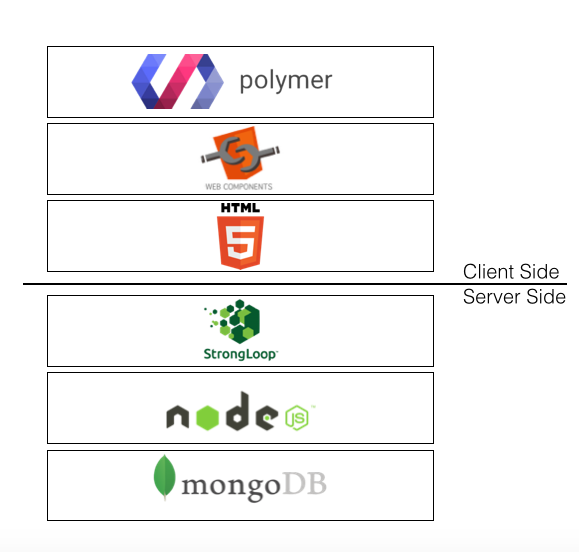
\includegraphics[width=1.0\linewidth]{images/chapter4/XPR_stack.png}\hfill
 \caption[X-learning Architectural Stack]{X-Learning Architectural Stack}
 \label{fig:fourV}
\end{figure}

\subsubsection {1st step - Models schemas definition}
\label{subsec:1st_step_models_schemas_definitio}


A description of entities, properties, relations and data access policies are defined as JSON  documents.
As to a learning platform, the essential entities to be modelled are the following: Course, Lecture, Video and Teacher(Member).

\subsubsection{ Model - Member}

The model Member represents the course creator but also the students of other course. Its features are: name, lastname, email.gender,photo,phone number,location and date. The Member has relations with course, and for each of these relation can be learning or teaching.

\begin{lstlisting}[language=json]
{
  "name": "Member",
  "base": "User",
  "properties": {
    "name": {
      "type": "String"
    },
    "last_name": {
      "type": "String"
    },   
    "birthday": {
      "type": "Date"
    },
    "email": {
      "type": "String"
    },
    "gender": {
      "type": "String"
    },
    "password": {
      "type": "String"
    },
    "photo": {
      "type": "String"
    },
    "location": {
      "type": "String"
    },
    "phone": {
      "type": "Number"
    }
  },
  "relations": {
    "learning": {
      "type": "hasAndBelongsToMany",
      "model": "Course",
      "through": "MemberCourse"
    },
    "teaching": {
      "type": "hasMany",
      "model": "Course",
      "foreignKey": "teacher_id"
    }
  }
}
\end{lstlisting}


\subsubsection{ Model - Course}

The model Course defines the main element structure that must be published. Main features are: title, cost, documentation, publish and publication date. This model has relations with teacher, students, category, lectures and webinars models.


\begin{lstlisting}[language=json]
{
  "name": "Course",
   "properties": {
    "title": {
      "type": "String"
    },
    "description": {
      "type": "String"
    },
    "date": {
      "type": "Date"
    },
    "cover": {
      "type": "String"
    },
    "language": {
      "type": "String"
    },
    "cost": {
      "type": "Number"
    },
    "publish": {
      "type": "Boolean"
    },
    "documents": {
      "type": "Array"
    },
    "skill": {
      "type": "Array"
    }
  },
  "relations": {
    "category": {
      "type": "belongsTo",
      "model": "Category",
      "foreignKey": "category_id"
    },
    "teacher": {
      "type": "belongsTo",
      "model": "Member",
      "foreignKey": "teacher_id"
    },
    "lectures": {
      "type": "hasMany",
      "model": "Lecture",
      "foreignKey": "course_id"
    },
    "webinars": {
      "type": "hasMany",
      "model": "Webinar",
      "foreignKey": "webinar_id"
    },
    "students": {
      "type": "hasAndBelongsToMany",
      "model": "Member",
      "through": "MemberCourse"
    }

\end{lstlisting}

\subsubsection{ Model - Lecture}

The model Lecture defines the single lecture into a determinate course. Main features are: title, description. This model has relations with course, video.


\begin{lstlisting}[language=json]
{
  "name": "Lecture",
  "properties": {
    "title": {
      "type": "String"
    },
    "description": {
      "type": "String"
    }
  },
  "relations": {
    "course": {
      "type": "belongsTo",
      "model": "Course",
      "foreignKey": "course_id"
    },
    "video": {
      "type": "hasOne",
      "model": "Video",
      "foreignKey": "lecture_video_id"
    }
  }

\end{lstlisting}

\subsubsection{ Model - Video}

The model Video defines the video object belong to lecture. Main features are: title, url and duration of its. This model has relations with lecture.


\begin{lstlisting}[language=json]
{
  "name": "Video",
  "properties": {
    "title": {
      "type": "String"
    }
    "url": {
      "type": "String"
    },
    "duration": {
      "type": "Number"
    }
  },
  "relations": {
    "lecture": {
      "type": "belongsTo",
      "model": "Lecture",
      "foreignKey": "lecture_video_id"
    }
  }
}

\end{lstlisting}


\subsubsection {2nd step - HTTP RESTful API definition}
\label{subsec:2nd_step_HTTP_RESTful_API_definition}

CRUD operations on models are automatically generated by the web framework (on the basis of input JSON documents) and further custom actions can be defined. All of them are exposed as HTTP RESTful API.
These models result in the following HTTP RESTful API, automatically generated by Loopback server.

\subsubsection{ Members API}
\begin{itemize}
\item \textbf{GET /api/Members} Find all instances of the model matched by filter from  the  data source.
\item \textbf{POST /api/Members} Update an existing model instance or insert a new one into the data  source.
\item \textbf{PUT /api/Members} Create a new instance of the model and persist it into the data source.
\item \textbf{DELETE /api/Members/id} Delete a model instance by id from the data source.
\item \textbf{GET / Members/id/teaching} {\color{red}Queries teacher course of model.}

\item \textbf{GET / Members/id/learning} {\color{red} Queries follow course of model.}

\item \textbf{POST /api/changeEmail} Change email of a model instance.
\item \textbf{POST /api/changePassword} Change password of a model instance.
\item \textbf{GET /api/count Count} instances of the model matched by where from the  data source.
\item \textbf{POST /api/login} Login a user with username/email and password.
\item \textbf{POST /api/logout} Logout a user with access   token.
\item \textbf{POST /api/reset} Reset password for a user with email.
\item \textbf{POST /api/update} Update instances of the model matched by where from the data source.
\end{itemize}

\subsubsection{ Course API}
\begin{itemize}
\item \textbf{PUT /Courses} Update an existing model instance or insert a new one into the data  source.
\item \textbf{GET /Courses} Find all instances of the model matched by filter from the data  source.
\item \textbf{POST / Courses} create a new instance and persist it into the data source.
\item \textbf{GET / Courses/id/lectures} Queries lectures of course.
\item \textbf{POST / Courses/id/lectures} Creates a new instance in lectures of  this model.
\item \textbf{DELETE / Courses/id/lectures} Deletes all lectures of this model.

\item \textbf{GET / Courses/id/webinars} Queries webinars of course.
\item \textbf{POST / Courses/id/webinars} Creates a new instance in webinars of  this model.
\item \textbf{DELETE / Courses/id/webinars} Deletes all webinars of this model.

\item \textbf{GET / Courses/id/students} Queries students of course.
\item \textbf{POST / Courses/id/students} Creates a new instance in students of  this model.
\item \textbf{DELETE / Courses/id/students} Deletes all students of this model.
\end{itemize}


\subsubsection{ Lectures API}
\begin{itemize}
\item \textbf{GET /api/Lectures} Find all instances of the model matched by filter from  the  data source.
\item \textbf{POST /api/Lectures} Update an existing model instance or insert a new one into the data  source.
\item \textbf{PUT /api/Lectures} Create a new instance of the model and persist it into the data   source.
\item \textbf{DELETE /api/Lectures/id} Delete a model instance by id from the data source.
\item \textbf{GET /api/Lectures/id/course} Fetches belongsTO relation course.

\item \textbf{GET /api/Lectures/id/video} Fetches belongsTO relation video.
\item \textbf{GET /api/Lectures/count} Count instances of the model matched by where from the data  source.
\end{itemize}

\subsubsection{ Images API}

\begin{itemize}
\item \textbf{POST /Model}
\item \textbf{POST /Images} create a new instance and persist it into the data source.
\item \textbf{PUT /Images} Update an existing model instance or insert a new one into the data source.
\item \textbf{GET /Images} Find all instances of the model matched by filter from the  data source.
\item \textbf{POST /Images/upload} Upload a new instance into data source.
\item \textbf{GET /Images/id} Find a model instance by id from the data source
\item \textbf{PUT /Images/id} Update attributes of a model instance and persist it into the data source.
\item \textbf{DELETE /Images/id} Deletes a model instance by id from the data 
source.
\end{itemize}

\subsubsection{ Videos API}
\begin{itemize}
\item \textbf{POST /Videos} create a new instance and persist it into the data source.
\item \textbf{PUT /Videos} Update an existing model instance or insert a new one into the data source.
\item \textbf{GET /Videos} Find all instances of the model matched by filter from the  data source.
\item \textbf{GET /Videos/id} Find a model instance by id from the data source
\item \textbf{PUT /Videos/id} Update attributes of a model instance and persist it into the data source.
\item \textbf{DELETE /Videos/id} Deletes a model instance by id from the data 
source. 
\item \textbf{GET /Videos/id/lecture} Fetches belongsTO relation lecture.
\end{itemize}

\subsubsection{Webinars API}
\begin{itemize}
\item \textbf{POST /Webinars} create a new instance and persist it into the data source.
\item \textbf{PUT /Webinars} Update an existing model instance or insert a new one into the data source.
\item \textbf{GET /Webinars} Find all instances of the model matched by filter from the  data source.
\item \textbf{POST /Webinars/course} Fetches belongsTO relation course.
\item \textbf{GET /Webinars/id} Find a model instance by id from the data source
\item \textbf{PUT /Webinars/id} Update attributes of a model instance and persist it into the data source.
\item \textbf{DELETE /Webinars/id} Deletes a model instance by id from the data 
source.
\end{itemize}

 \subsubsection{ Remote Methods }
  
  Come abbiamo detto per ogni modello vengono generate automaticamente le api dal server di Strongloop. Ogni modello rappresentato da un file JSON è anche accompagnato da un file js che di default si presenta in questo modo definito come hook
  \begin{lstlisting}[language=javascript]

    module.exports = function (x-model) {
    
    };
  \end{lstlisting}


Use model hooks to add custom logic to models that extend PersistedModel. Each hook is called before or after a specific event in the model's lifecycle.
Best practice is to register model hooks in /common/models/x-model.js
Di seguito sono riportate alcuni metodi remoti che sono stati creati e un esempio esplicativo.

\begin{itemize}
\item \textbf{GET /videos/signed\_upload\_part }
\item \textbf{GET /videos/create\_multiPart\_upload}
\item \textbf{PUT /videos/complete\_upload\_part }
\item \textbf{DELETE /videos/delete\_video}
\end{itemize}

\begin{lstlisting}[language=javascript]

module.exports = function (Video) {
  ...
Video.delete_video = function(path,callback) {
    var self = this;
    var params = {
      Bucket: S3_BUCKET,
      Prefix: path
    };

    s3.listObjects(params, function(err, data) {
      if (err){
        console.log(err);
        callback(err);
        return;
      } 

      params = {Bucket: S3_BUCKET};
      params.Delete = {};
      params.Delete.Objects = [];

      data.Contents.forEach(function(content) {
        params.Delete.Objects.push({Key: content.Key});
      });

      s3.deleteObjects(params, function (err, delete_response) {
        if (err){
          console.log(err);
          callback(err);
          return;
        }

        console.log(delete_response.Deleted.length);
        callback(null, delete_response);
      });
    });
  };

  Video.remoteMethod('delete_video', {
    http: { verb: 'delete' },
    accepts: [
      {arg: 'path', type: 'string'}
    ],
    returns: {arg: 'delete_response', type: 'string'}
  });
  ....
};
\end{lstlisting}

\subsubsection {3rd step - UI components definition}
\label{subsec:3rd_step_UI_components_definition}

Distinct UI components can be defined, or retrieved from a collection of predefined components, configured and adapted. They represent the building blocks of the whole UI.
{\color{red}The following is an example:}

\begin{lstlisting}[language=html]
<part-course-actions course="{{course}}"></part-course-actions>
\end{lstlisting}

\begin{figure}[htb] %  figure placement: here, top, bottom
 \centering
 
\includegraphics[width=1.0\linewidth]{images/chapter4/admin-course-actions.png}\hfill
 \caption[Page Admin course action]{Page Admin course action}
 \label{fig:fourV}
\end{figure}

\begin{lstlisting}[language=html]
<part-course-info course="{{course}}" error="{{error}}"></part-course-info>
\end{lstlisting}


\begin{figure}[htb] %  figure placement: here, top, bottom
 \centering
 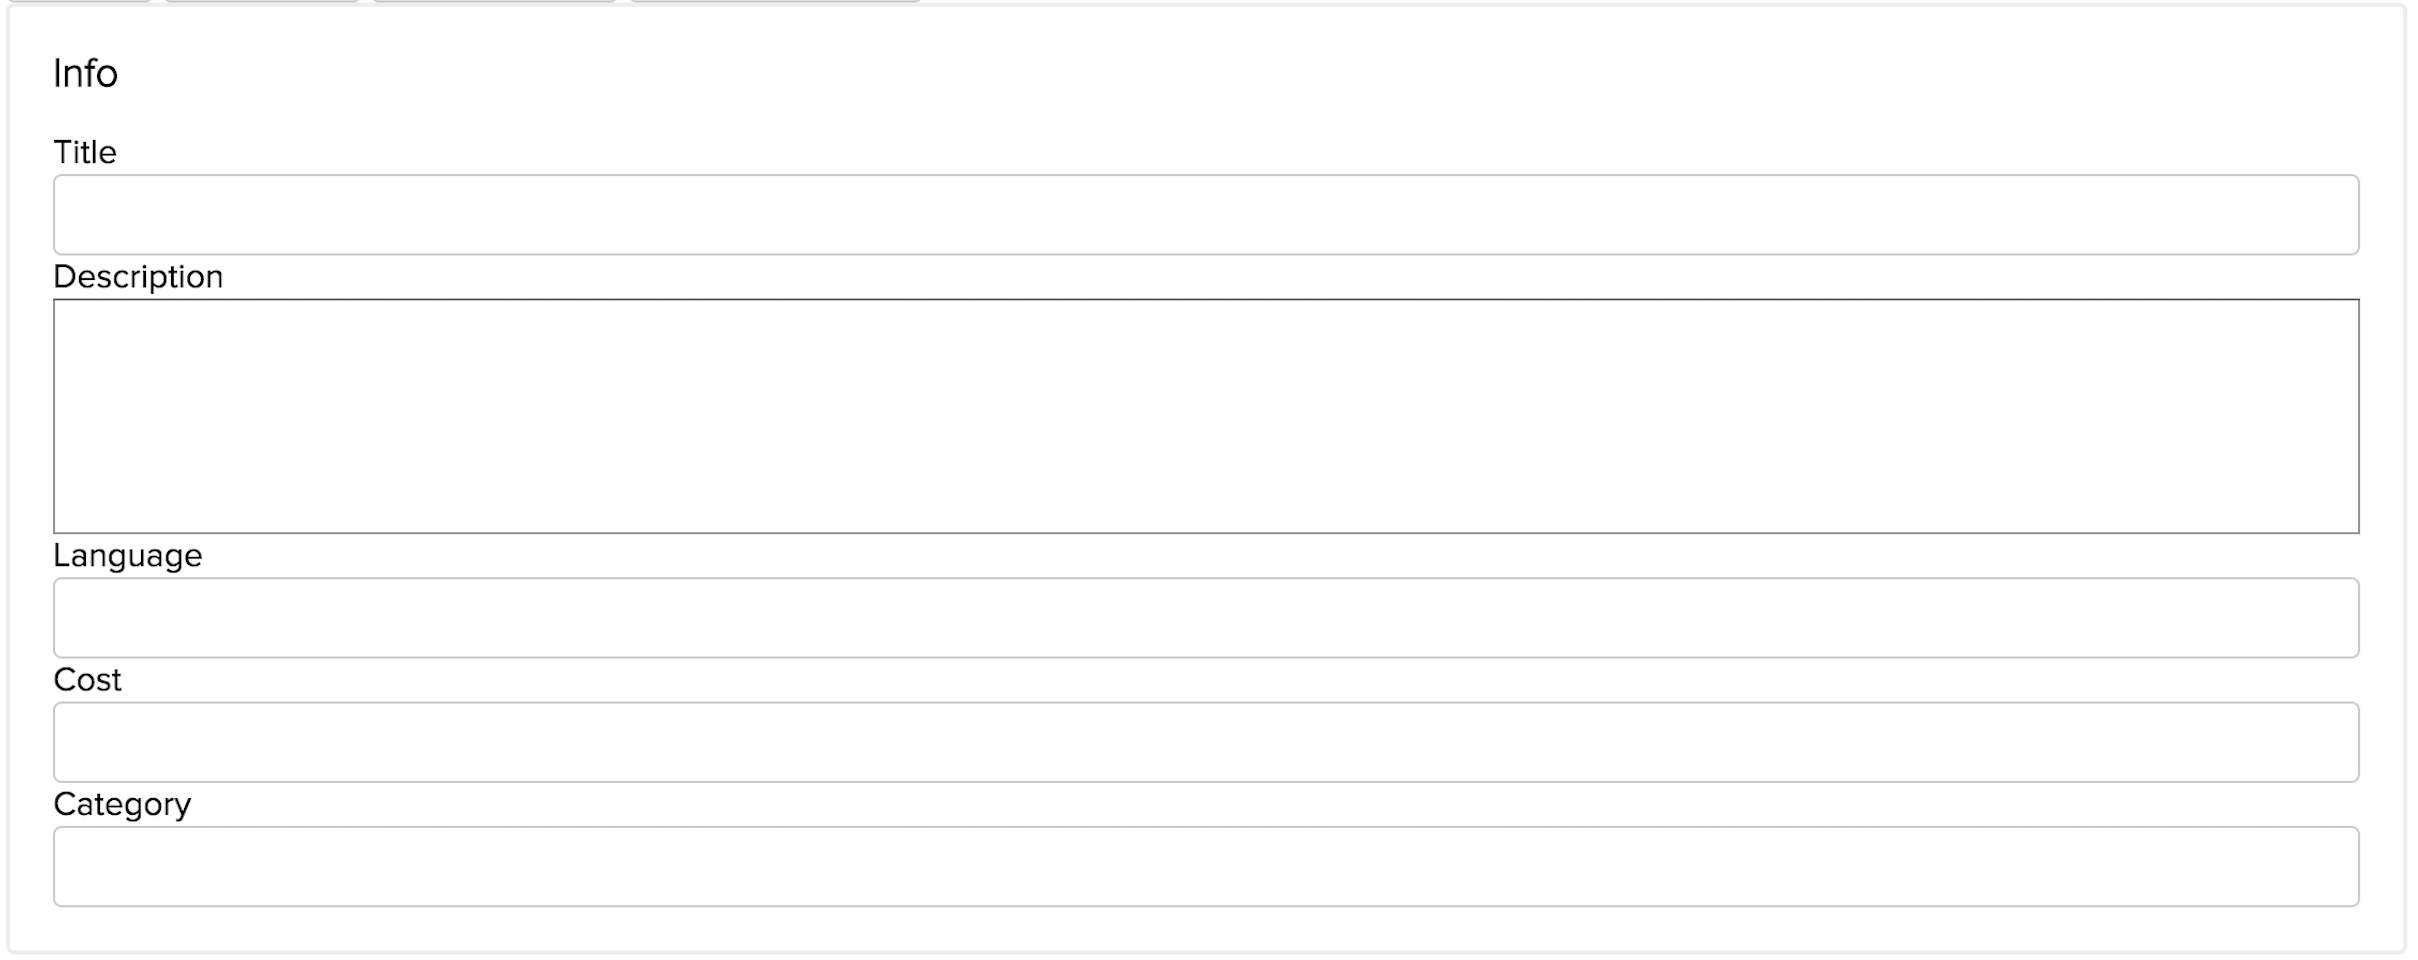
\includegraphics[width=1.0\linewidth]{images/chapter4/admin-course-info.png}\hfill
 \caption[Page Admin course info]{Page Admin course info}
 \label{fig:fourV}
\end{figure}

\subsubsection {4th step - UI components assembly}
\label{subsec:4th_step_UI_components_assembly}

Distinct UI components are finally mounted to compose the application views. Assembly is kept as simple as possible: it only consists of a composition of HTML5 elements. So, the entire development process results driven by: JSON documents describing entities of the application and HTML template documents describing the UI components.

\begin{figure}[htb] %  figure placement: here, top, bottom
 \centering
 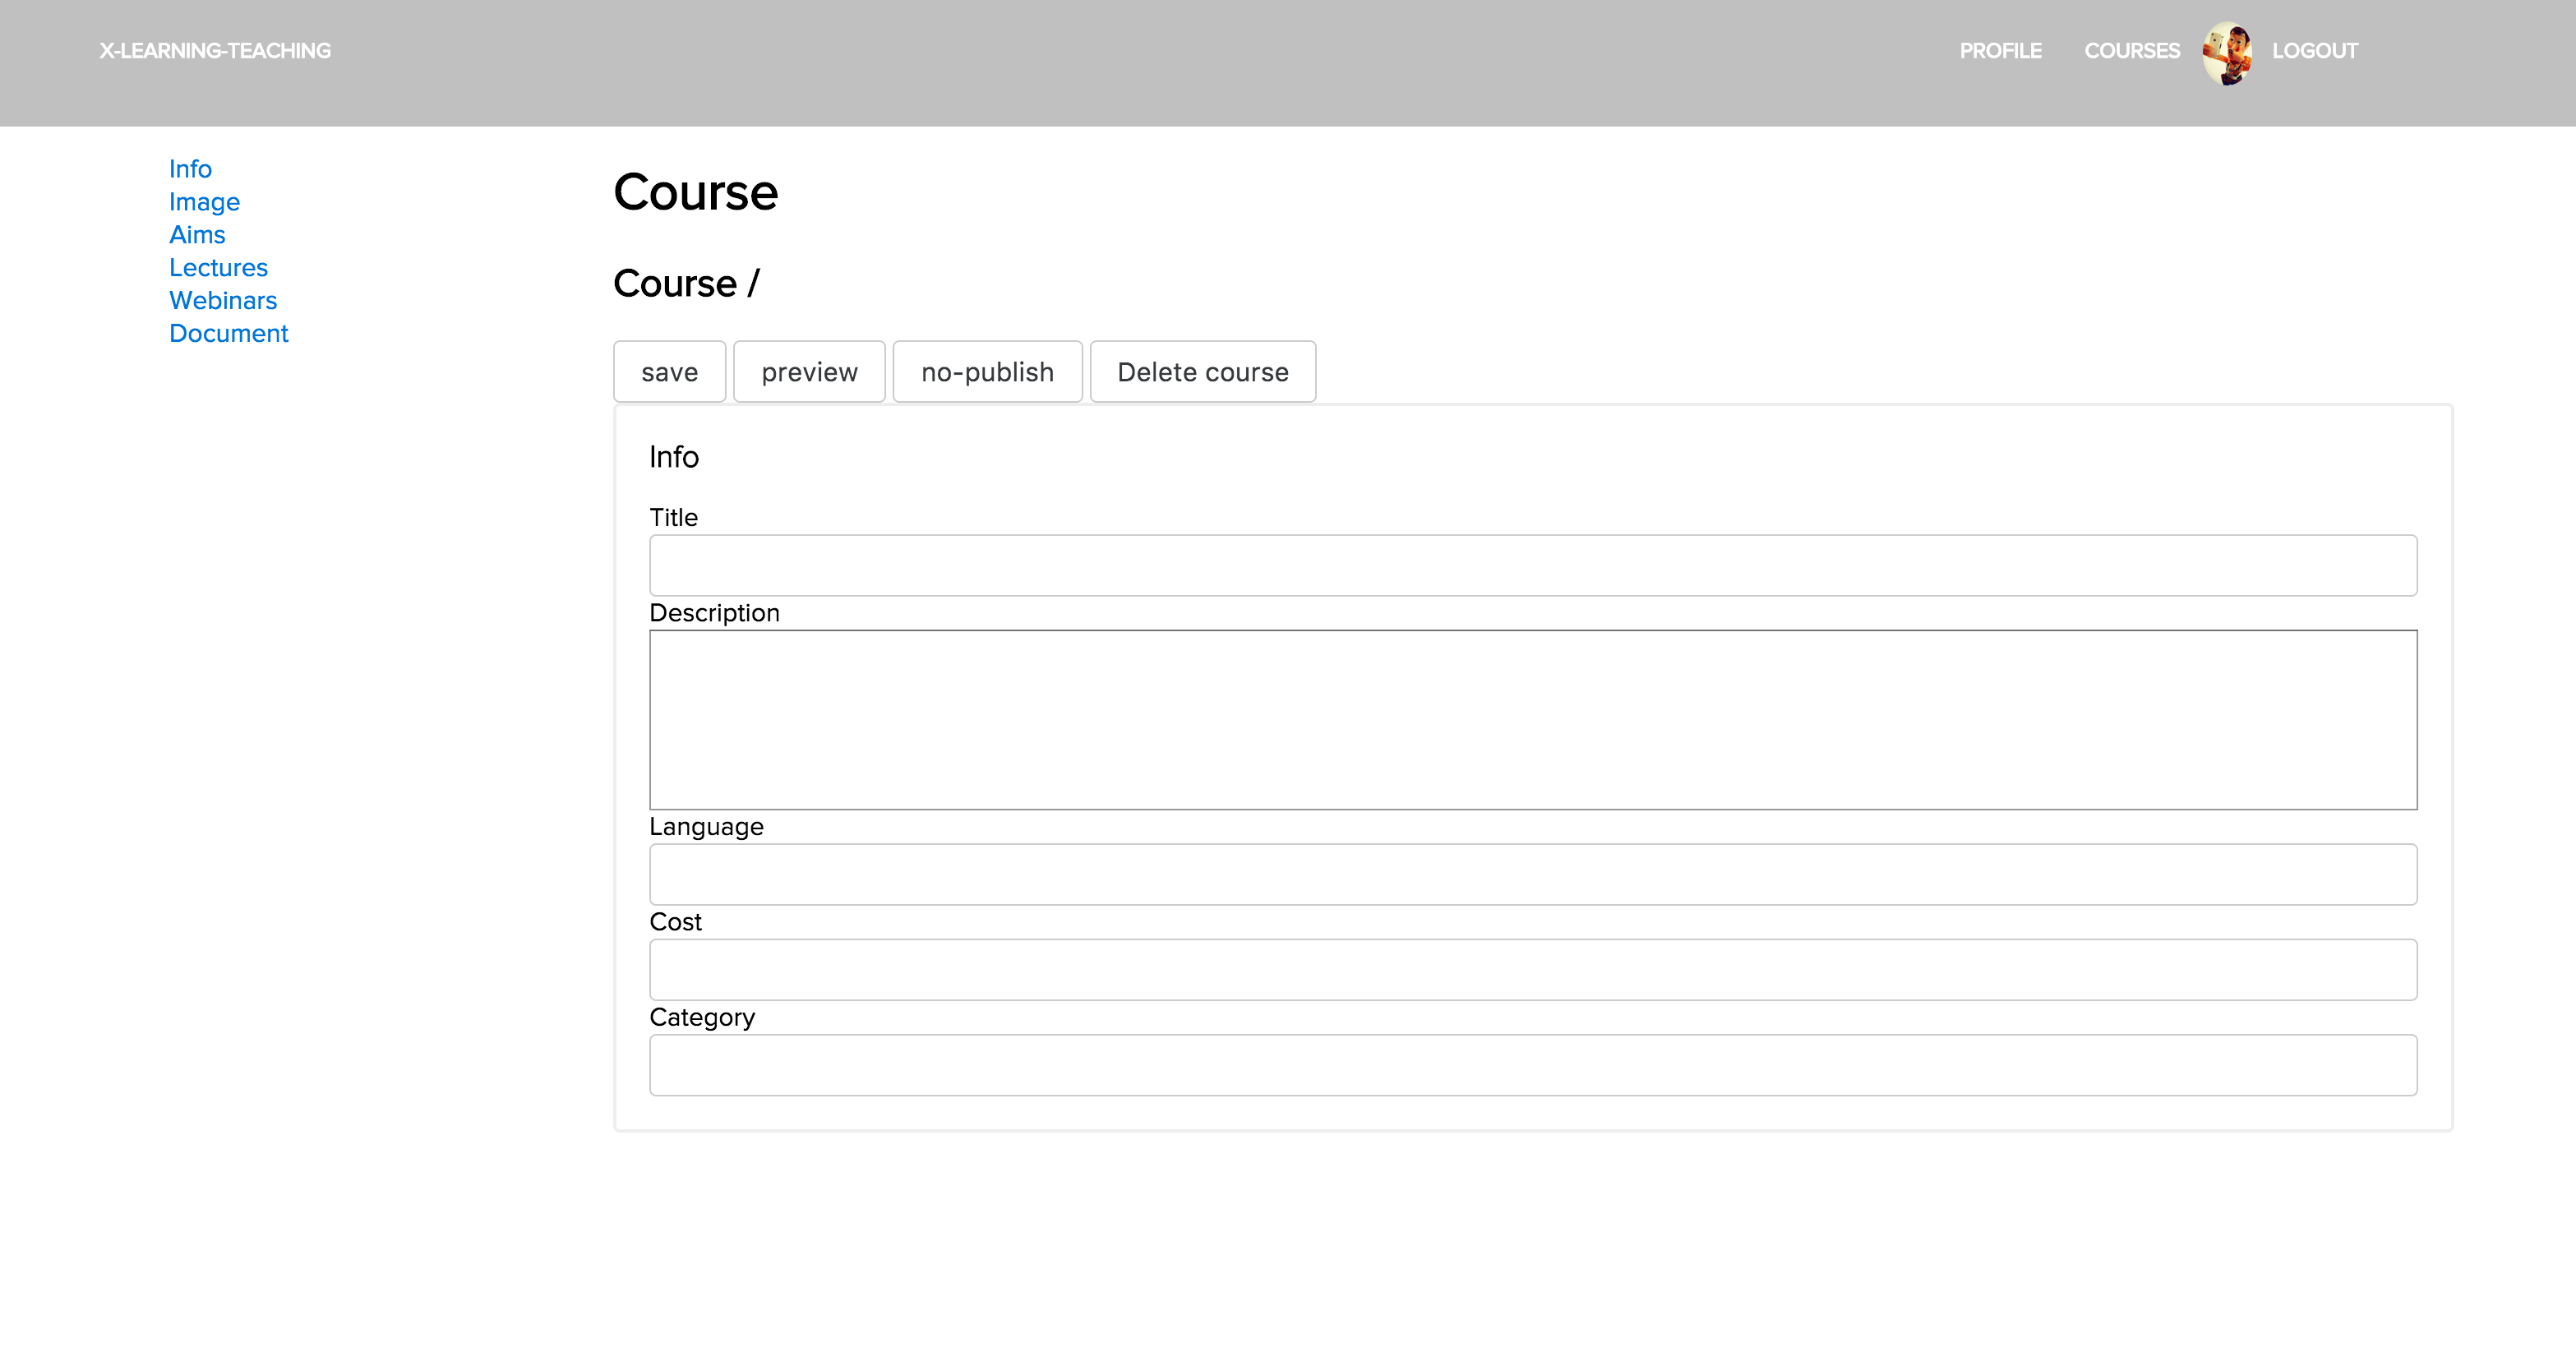
\includegraphics[width=1.0\linewidth]{images/chapter4/admin-course.png}\hfill
 \caption[Page Admin course]{Page Admin course}
 \label{fig:fourV}
\end{figure}






\chapter{Video Management:?}
\label{cha:chapter_5_a}

In this chapter...

\section{Section 1}
\label{sec:chapter_5_a_section_1}

In this section...

\section{Section 2}
\label{sec:chapter_5_a_section_2}

In this section...




\chapter{Chapter 5 B}
\label{cha:chapter_5_b}

In this chapter...

\section{Section 1}
\label{sec:chapter_5_b_section_1}

In this section...

\section{Section 2}
\label{sec:chapter_5_b_section_2}

In this section...

In conclusions...



\newpage

\chapter{Conclusions}
\label{cha:conclusions}

\section{Work performed}
\label{sec:work_performed}
 
In conclusione sono state gettate le basi per un progetto ambizioso che consente a un utente di realizzare la propria piattaforma di e-learning.

In X-Learning il caso d'uso analizzato, sono stati sfruttati i benifici lato client derivanti da Polymer e Web Components, Server-side benefits are represented by the easy way of API creation through model definitions.
Code reusability and access to reusable code are, clearly, one of the most important aspects of the project that lead to the implementation of a set of elements.

I componenti principali creati durante il progetto di tesi sono certamente quelli utili alla gestione e allo streaming dei contenuti video su cui si basa l'intera piattaforma.

Sono quindi stati creati diversi elementi stand alone che incapsulano l'intera complessità e che possono essere riutilizzati in diversi contesti e progetti.

L'interazione tra i vari servizi quali multiPartUpload, Elastic Transcoder, SQN, Cloufront è stata possibile grazie all'utilizzo delle diverse API messe a disposizione.
E' risultato quindi di fondamentale importanza lo studio approfondito dei vari servizi Amazon AWS che ha reso possibile la realizzione di tali componenti.
% Attraverso l'utilizzo delle diverse API  e quindi 

Inoltre è stato necessario approfondire anche lo studio dello standard w3c WebRTC e della libreria PeerJS che ha reso possibile la realizzazione di componenti stand alone che permettono la comunicazione peer to peer, sfruttata in X-Learning per ampliare l'offerta dei corsi con l'aggiunta dei Webinar.

\section{Future developments}
\label{sec:future_developments}

Al momento il caso d'uso X-learning è in uno stato molto avanzato ma ancora non definitivo del progetto che si vuole portare a termine.
Per questo sono già stati identificati alcuni punti da cui ripartire per poter rendere definitivamente disponibile un servizio completo e allo stesso tempo pronto ad offrire la possibilità di creare una propria piattaforma.

Tra gli sviluppi futuri sicuramente il principale è il deploy, ovvero incapsulare tutta la piattaforma creando uno strato superiore che per ogni utente istanzi una macchina Docker dedicata e già preconfigurata con all'interno tutte le tecnologie necessarie.

Di seguito sono riportati i principali obiettivi che in ottica futura renderebbero il progetto intrapeso definitivmente completo.

\begin{itemize}
  \item Integrare la piattaforma, con servizi offerti dalle piu comuni piattaforme MOOC come ad esempio forum e chat tra utenti iscritti agli stessi corsi.

  \item Effettuare il porting da loopback a forester, ovvero un framework sviluppato all'interno del CVDLAB, che guarda al futuro sfruttando tecnologie moderne e non ancora particolarmente diffuse come koajs e le async/await ma che diventeranno ben presto essenziali. 

  \item Creare nuovi temi concedendo massima autonomia agli utenti di scegliere il tema più consono al stile della loro piattaforma.

  \item Use Adobe PhoneGap framework which is an open source distribution of Cordova that allow to quickly make hybrid applications.

  % Infine creare un app nativa desktop attraverso l'utilizzo di ELECTRON.
  \item Finally, through the Electron use, which is open source, maintained by GitHub and an active community, allow to build cross platform desktop apps with web technologies.\cite{electron}

\end{itemize}




\newpage

\part{Appendix}

\appendix

\chapter{Appendix 1}
\label{cha:appendix_1}


In this appendix...

This is the appendix.

\chapter{Appendix 2}
\label{cha:appendix_2}


In this appendix...

This is the appendix.

\newpage

% BibTex

%\nocite{*}

%\bibliographystyle{unsrt}

\cleardoublepage

\addcontentsline{toc}{chapter}{Bibliography}

\printbibliography

\input{tex_files/bibliography/bibliography}

\end{document}